%Cody Lewis, Luke De Ruyter, 2012
%Visit anzhelka.com for all the latest
%
% CTRL+SPACE to switch panes in Texmaker
%
% Note: blank lines indicate a new paragraph
% Note: \left( and \right) cannot break lines.

% NOTES: 
% --- Titles overlap for Engineering Effort and Societal Impacts.

% TODO: Additional material
% --- System design could be expanded (but not absolutely necessary

\documentclass{article}

% Packages that are being used.
\usepackage{amsmath}
\usepackage{longtable}
\usepackage{color}
%\usepackage{verbatim} % used to display code
\usepackage{listings}
\usepackage{graphicx}
\usepackage{subfigure}
\usepackage{indentfirst}
\usepackage{fancyhdr} % Fancy Header
\usepackage{rotating} % To make vertical text in tables
\usepackage[normalem]{ulem} %for strikethroughs


\usepackage{hyperref} %Must be at the end of use package but before "other settings". Used to make links of all references.




\numberwithin{equation}{section} %change the numbering to have something like 1.1 and 3.15, etc.
%Format of macro:
%\newcommand{\NAME}[ARGUMENT NUMBER (OPTIONAL)]{ stuff to include, arguments denoted #1, #2, etc. }
\newcommand{\vect}[1]{\boldsymbol{#1^2}}
\newcommand{\bigvect}[3]{\boldsymbol{#1^#2^#3}}
\newcommand{\bs}[1]{\boldsymbol{#1}}

\definecolor{lightlightgray}{gray}{0.9}

\graphicspath{{../tests/}{../figures/}{../extra/}} %\graphicspath{{path/one/}{path/two/}{path/three/}}

\fancyfoot[CO,CE]{ \thepage \\ 
\includegraphics[width=2cm]{../extra/pheonix_small.png}}
\pagestyle{fancy}



\begin{document}



\lstset{
%language=C,                             % Code langugage
basicstyle=\ttfamily,                   % Code font, Examples: \footnotesize, \ttfamily
keywordstyle=\color{OliveGreen},        % Keywords font ('*' = uppercase)
commentstyle=\color{gray},              % Comments font
%numbers=left,                           % Line nums position
%numberstyle=\tiny,                      % Line-numbers fonts
%stepnumber=1,                           % Step between two line-numbers
%numbersep=5pt,                          % How far are line-numbers from code
backgroundcolor=\color{lightlightgray}, % Choose background color
frame=none,                             % A frame around the code
tabsize=4,                              % Default tab size
captionpos=b,                           % Caption-position = bottom
breaklines=true,                        % Automatic line breaking?
breakatwhitespace=false,                % Automatic breaks only at whitespace?
showspaces=false,                       % Dont make spaces visible
showtabs=false,                         % Dont make tabls visible
%columns=flexible,                       % Column format
%morekeywords={__global__, __device__},  % CUDA specific keywords
}








\title{\Huge Autonomous Quadrotor Project}
\author{Cody Lewis \\ \texttt{srlm@anzhelka.com} \and Luke De Ruyter \\ \texttt{ilukester@anzhelka.com} }
\date{\today}
\maketitle 
\begin{center}
\includegraphics[scale=.24]{tribal_phoenix.jpg}\end{center}
\bigskip \bigskip \bigskip \bigskip \bigskip \bigskip \bigskip \bigskip \bigskip \bigskip
\begin{verse}\textit{
And when he [Herod] had apprehended him [Peter], he put him in prison, and delivered him to four quaternions of soldiers to keep him; intending after Easter to bring him forth to the people.} \\
\hfill --Acts 12:14, King James Bible, Cambridge Edition
\end{verse}



%% REV REV REV REV REV REV REV REV REV REV REV REV REV
\newpage
\addcontentsline{toc}{section}{Abstract}
%\begin{abstract}
\section*{Abstract}
This project discusses the design of a four rotor autonomous aerial vehicle platform called the Anzhelka Project. The system is based on the open source Elev-8 quadrotor mechanical hardware platform and the Parallax P8X32A microcontroller. In this paper we discuss the preparation that we have done in order to create a stable, autonomous vehicle. We then propose an implementation sequence that will result in a stable, autonomous hover. This paper focuses on the practical aspects of quadrotor flight. For a theoretical treatment see the Anzhelka project mathematics document \cite{anzhelka_math}.
%\end{abstract}

\addcontentsline{toc}{section}{Revisions}
\section*{Revisions}
Current project status and files can be found at
\begin{center}
\bigskip \textbf{blog.anzhelka.com} \\
 \textbf{code.anzhelka.com} \\
 \bigskip
\end{center}

\begin{longtable}{l | p{5cm} | l}
\hline
\textbf{Version} & \textbf{Changes} & \textbf{Commiter}\\
\hline
v0.01 & All of the spelling was checked and fixed for the first 2 sections. & Luke \\
\hline
v0.02 & Needs to be proof read in some areas. Needs tables, conclusions, High level, references, appendices, acknowledgements & Luke \\
\hline
v0.03 & Cleaned up the document some, added images and tables. & Cody \\
\hline
v0.04 & Added conclusion, estimated control loop speed, small sections, figures. & Cody \\
\hline
v0.05 & Fixed some gramtical errors, added weights, cleaned up. & Luke \\
\hline
\end{longtable}

%% REV REV REV REV REV REV REV REV REV REV REV REV REV

%% TOC TOC TOC TOC TOC TOC TOC TOC TOC TOC TOC TOC
\newpage
\renewcommand{\contentsname}{Table of Contents}
\tableofcontents
\addcontentsline{toc}{section}{Table of Contents}
\newpage
%% TOC TOC TOC TOC TOC TOC TOC TOC TOC TOC TOC TOC

%% S1 S1 S1 S1 S1 S1 S1 S1 S1 S1 S1 S1 S1 S1 S1 S1 S1 S1 S1 S1  

%% S1 S1 S1 S1 S1 S1 S1 S1 S1 S1 S1 S1 S1 S1 S1 S1 S1 S1 S1 S1  

%% S1 S1 S1 S1 S1 S1 S1 S1 S1 S1 S1 S1 S1 S1 S1 S1 S1 S1 S1 S1  
\section{Executive Summary}
\begin{figure}[h!]
  \centering
	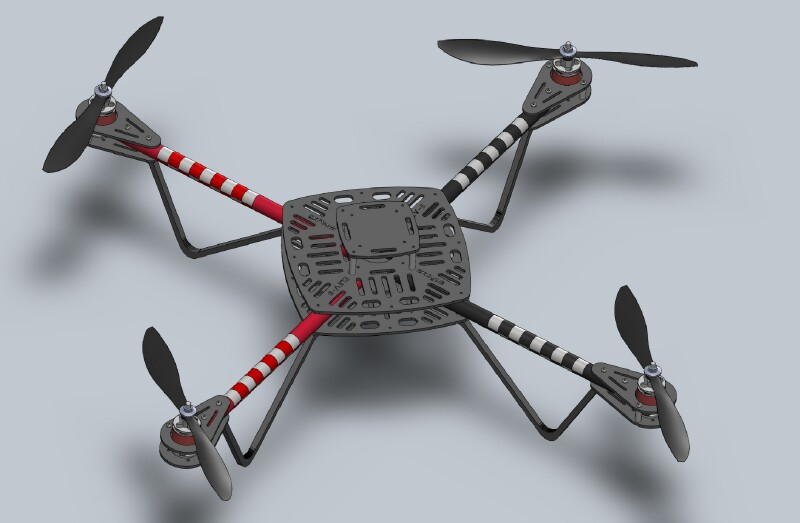
\includegraphics[scale=.6]{elev_8_rendering.JPG}
  \caption{Rendering of the Open Source Elev-8 quadrotor platform used in the Anzhelka project (image courtesy of Parallax).}
\end{figure}  

This senior design project's goal is to create an autonomous quadrotor that can be used to film outdoor sports such as mountain biking, snowboarding, and skiing. The quadrotor will have a video camera mounted on a gimbal that will always point at a subject/object to which the tracking device is attached. The tracking device will have its own GPS and IMU in order to be able to determine the location and heading of the subject/object. The quadrotor is intended to fly autonomously, ie without a human controller. The quadrotor should be able to maintain attitude (orientation) and position without human intervention.

Our quadrotor has many features including: 
\begin{list}{*}{}
	\item 3-axis gyro
	\item 3-axis accelerometer
	\item 3-axis compass
	\item voltage and current monitoring of each motor
	\item a separate battery for logic operations
	\item the ability to control up to 8 servos
	\item the ability to track the exact speed of each motor
	\item 8 unallocated analog inputs
	\item mounting holes for all components and future upgrades
\end{list}

This senior design project was built around being Open. How Open? Both Open Source and Open Hardware. The open source frame that was used for the quadrotor was designed by Ken Gracey, an employee at Parallax, and is called the "Elev-8". Our project is hosted hosted by Google Code in the form of a Git repository (\cite{anzhelka_code}). Here you can find all the information used and created during this senior design project. There is also a blog which goes into some of the extensive detail that was put into this project (\cite{anzhelka_blog}). The main processing board for this quad rotor features a Parallax Propeller \footnote{The coincidence between Propeller and propeller is unfortunate and can be a source of confusion. If Propeller is capitalized then the text is referring to the Parallax microcontroller. If propeller is not capitalized then the text is referring to a fixed pitch airplane "air screw"}, overclocked to 100Mhz, and a fully custom board that measures in at 4 inches by 3 inches.

Testing the quadrotor is a challenge in and of itself. But before that, one of the tests that has to be done is to calculate some of the constants for the control algorithms (motor torque and thrust). This means that there must be a test stand that tests and can calculate both of these constants. A slightly different kind of test is testing the functionality of the control board that was designed for the quadrotor.

The project was started without any expertise or experience with autonomous flying or quadrotors, but with a will to learn, create and develop a system that could even be understood by anyone. Software is our group expertise. Both team members have years of experience in multiple programming languages. 

Hardware on the other hand is a bit more difficult. Only one team member has any experience with designing PCBs and circuits, but not nothing to the extent of this project. We believe that, based on the work we have put into the project, that we have earned the class credits that we are receiving. Approximately 30 hours per person per week were devoted to this project(terminal program).
%% S1 S1 S1 S1 S1 S1 S1 S1 S1 S1 S1 S1 S1 S1 S1 S1 S1 S1 S1 S1  

%% S1 S1 S1 S1 S1 S1 S1 S1 S1 S1 S1 S1 S1 S1 S1 S1 S1 S1 S1 S1  
\section{Introduction}

A quadrotor, also known as a quadrotor helicopter or quadcopter, is a mutltirotor aerial vehicle that has four rotors mounted on a rigid frame to provide lift. Quadrotor designs first appeared in the 1920s, but were abandoned because of bad performance and high pilot work load.

In order to keep a quadrotor from spinning on its own axis, it must be built with counter rotating blades. Without counter rotating blades the quadrotor would create enough torque to spin in a constant direction around its' own axis.

\begin{figure}[h!]
  \centering
	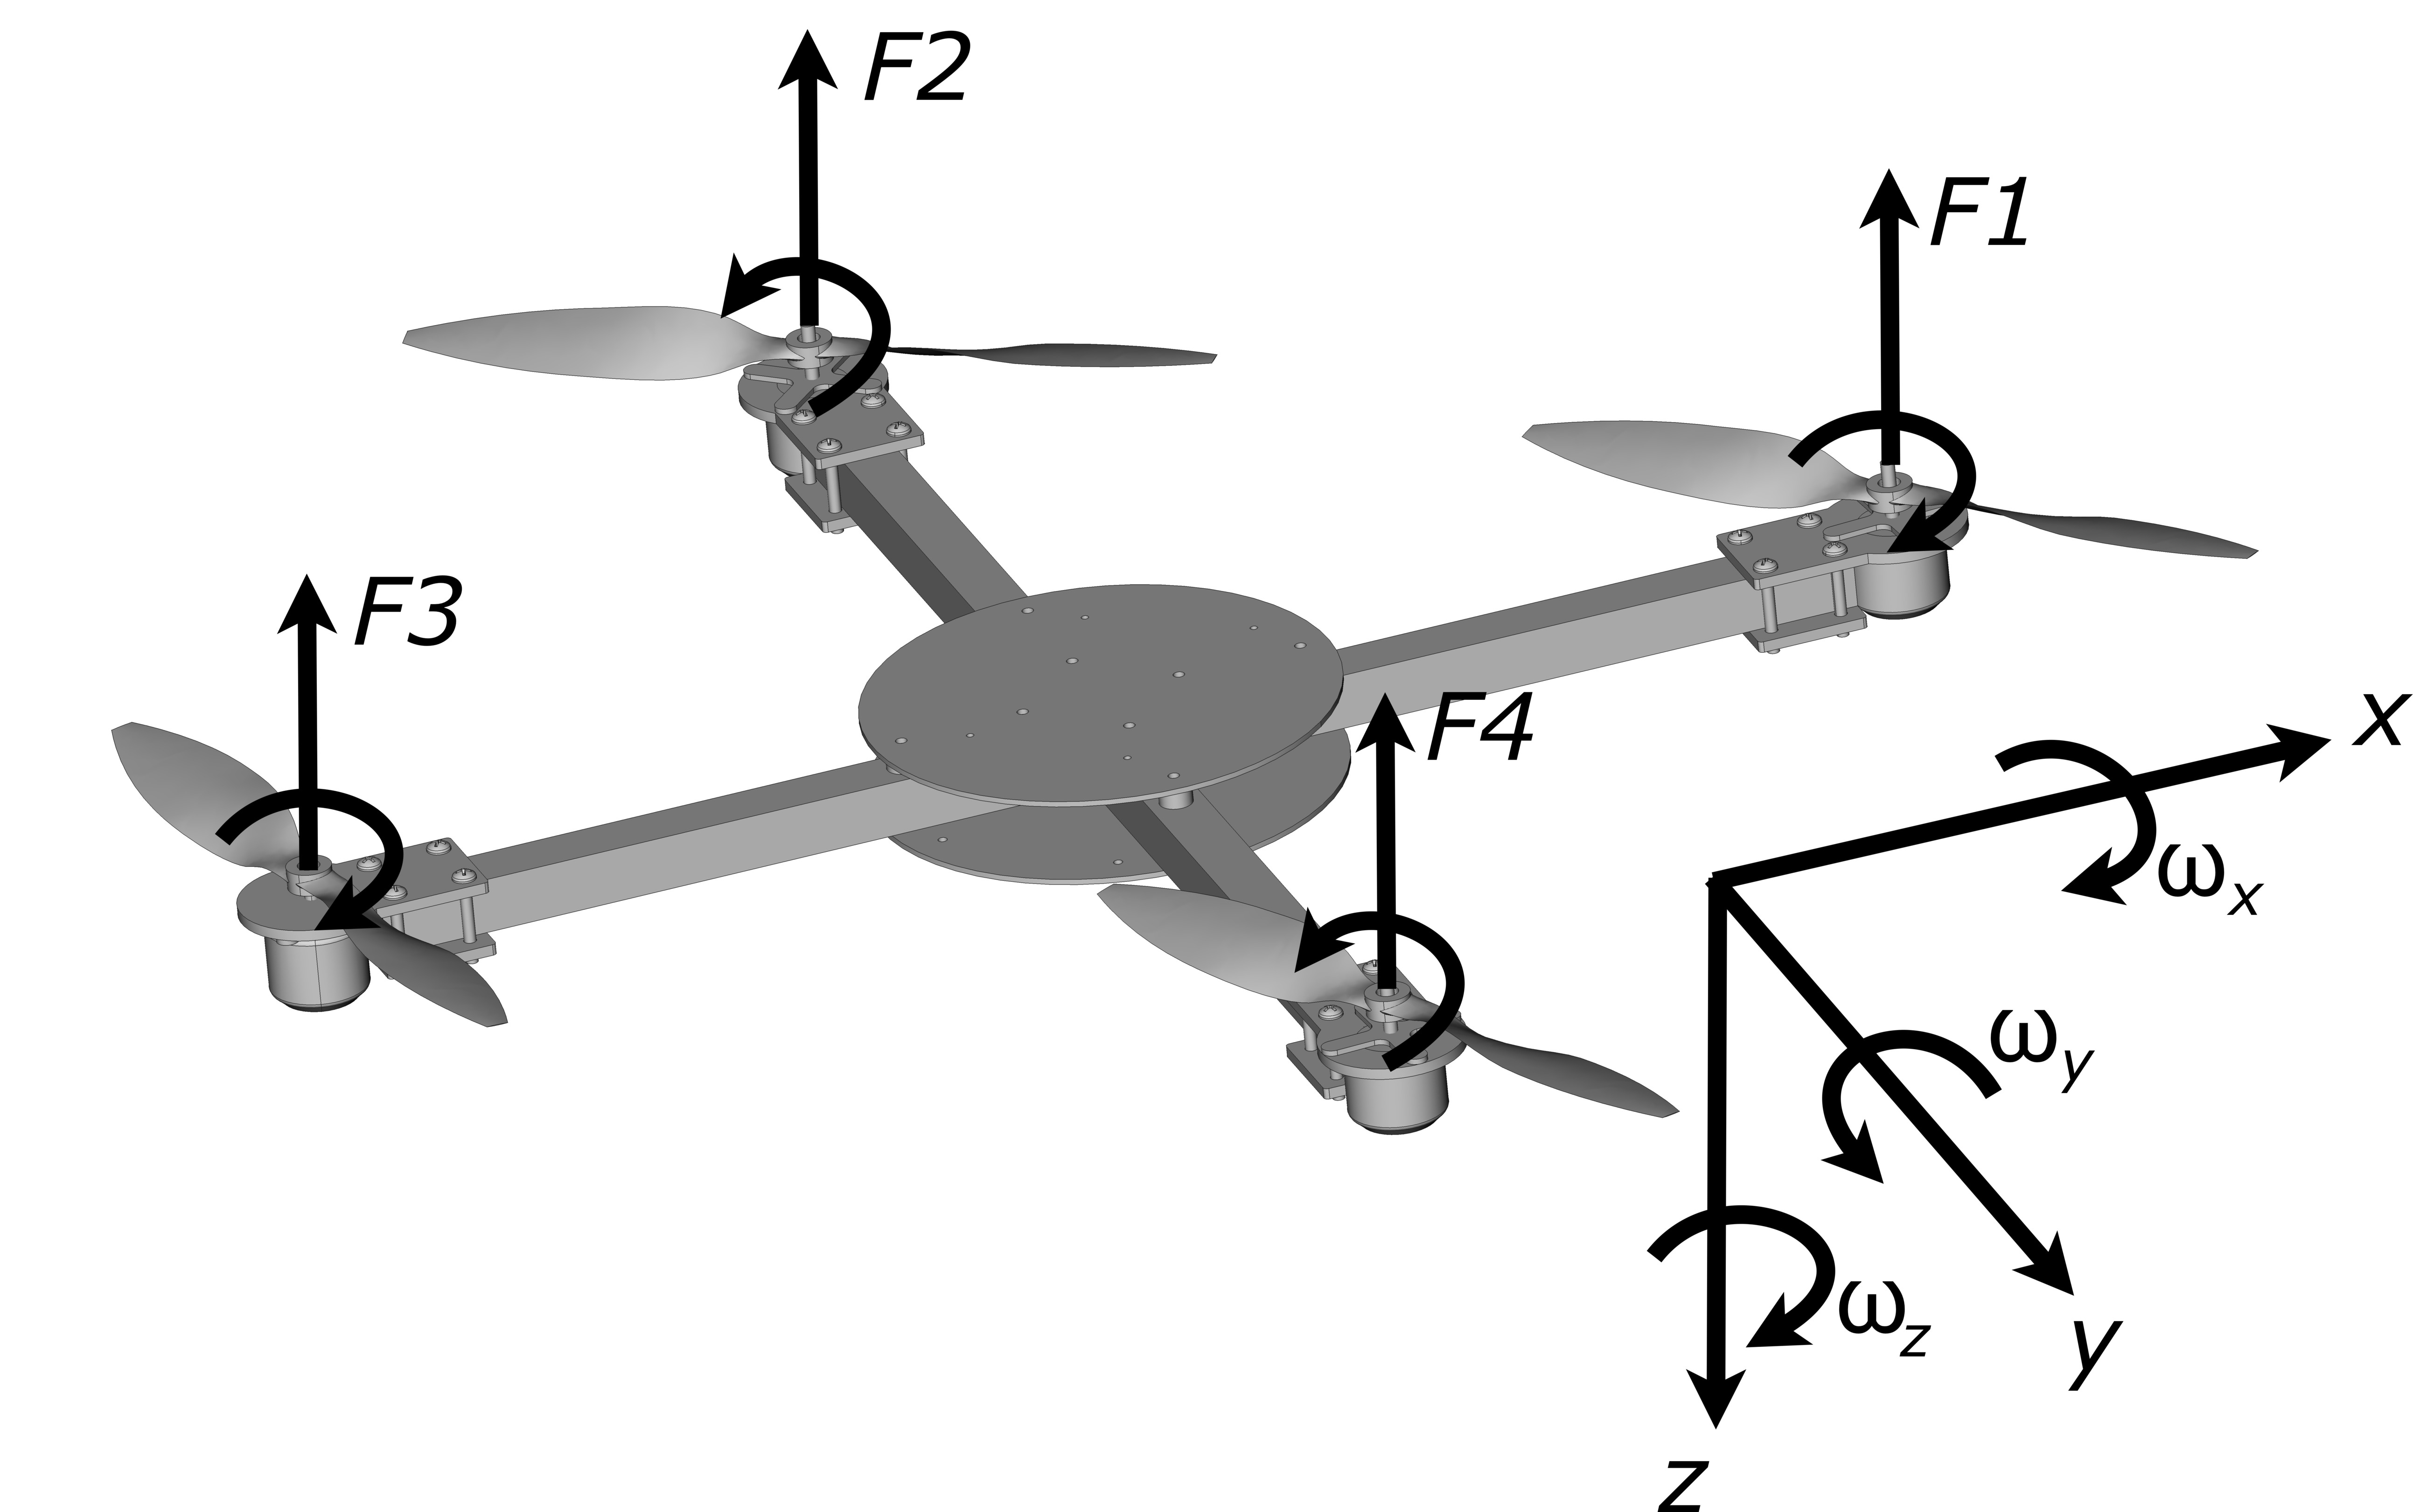
\includegraphics[scale=.05]{reference_frame_diagram.jpg}
  \caption{Orientation of the body axis with respect to the motor numbers and rotations.}
\end{figure}  

Quadrotors are highly manoeuvrable. A quadrotor can take off and land vertically. They can translate horizontally through the air, and they can also hold altitude. With a suitable pilot(or software) behind the controls one can do amzing aerial acrobatics with the quadrotor.

Quadrotors are very similar to helicopters, so what advantages do quadrotors have? Quadrotors have no mechanical gears between the motors and propellers. Each motor is directly driving its propeller. Having four propellers allows you to have a much smaller propeller than what is on the typical helicopter. This means that the propellers possess less kinetic energy while spinning allowing for a safer platform.
%% S1 S1 S1 S1 S1 S1 S1 S1 S1 S1 S1 S1 S1 S1 S1 S1 S1 S1 S1 S1  

\subsection{Quadrotor Mathematics}
A quadrotor is a very complex vehicle that is difficult to control. It is an under-actuated system with only one direction of force and three moment directions. The treatment of the math is too complex to include here. Instead, we have a separate document that discusses the math and theory of quadrotor flight in great detail. See citation \cite{anzhelka_math}. The rest of this paper will focus on everything else related to the quadrotor.

%% S2 S2 S2 S2 S2 S2 S2 S2 S2 S2 S2 S2 S2 S2 S2 S2 S2 S2 S2 S2

%% S2 S2 S2 S2 S2 S2 S2 S2 S2 S2 S2 S2 S2 S2 S2 S2 S2 S2 S2 S2  
\subsection{Design Objectives and System Overview}

This project was designed to be continuously improved upon and to be used in an many different ways. After watching countless videos from Go Pro cameras from a single perspectives and partial views of the subject, project Anzhelka was created. Anzhelka will allow users to be able to capture video angles that were once unattainable without costing thousands of dollars. Anzhelka will allow users to capture video with the same ease as using a Go Pro camera, but without the single perspective and jitter from traditional methods.

The quadrotor will have at least a 15 minute run time, with the ability to carry a 2 pound payload. It will also be optionally controllable by a human from up to a mile away with line of sight. The control loop to keep the platform stable will run at least 100Hz, enabling stable control.

On this project both team members share the same responsibility for all components of the system. This follows in the Agile philosophy. Each team member understands all aspects of the system, and has worked on all aspects. This creates a universal understanding a commitment to the project while removing territorial hoarding. There is no "my work", only "our work".
%% S2 S2 S2 S2 S2 S2 S2 S2 S2 S2 S2 S2 S2 S2 S2 S2 S2 S2 S2 S2  

\subsection{Current Project Status}
As of this writing, we still have work to do in order to achieve stable autonomous hover. We are in the process of testing the thrust torque test stand, and verifying all electrical circuits on the quadrotor. Once that is complete we will be able to write the three control loop blocks, as described in detail in the Anzhelka mathematics document \cite{anzhelka_math}. It is estimated that these blocks will be able to run at up to 300Hz (section \ref{subsec:codeperformanceestimation}).  For the project schedule, see subsection \ref{subsec:maintenance_plan_10}.

%% S2 S2 S2 S2 S2 S2 S2 S2 S2 S2 S2 S2 S2 S2 S2 S2 S2 S2 S2 S2  
\subsection{Background and Prior Art}
There are many different quadrotor designs available, but relatively few open source quadrotors. The most noticeable are the AeroQuad (\cite{aeroquad}) and the Arducopter (\cite{arducopter}). Most quadrotor theory seems to be the product of research labs such as \cite{stingu09}. This project is different in that it uses the Parallax propeller as it's processor and it is very well documented from the beginning.
%% S2 S2 S2 S2 S2 S2 S2 S2 S2 S2 S2 S2 S2 S2 S2 S2 S2 S2 S2 S2  

%% S2 S2 S2 S2 S2 S2 S2 S2 S2 S2 S2 S2 S2 S2 S2 S2 S2 S2 S2 S2  
\subsection{Development Environment and Tools}
%% S2 S2 S2 S2 S2 S2 S2 S2 S2 S2 S2 S2 S2 S2 S2 S2 S2 S2 S2 S2  

The Anzhelka project software was developed for the most part using a Linux system. All code and other project files are hosted on the project Git repository (\cite{anzhelka_code}). The 
 code was written in Gedit, compiled and downloaded with the \texttt{BSTC} compiler, and interfaced with using \texttt{picocom}.


%% S3 S3 S3 S3 S3 S3 S3 S3 S3 S3 S3 S3 S3 S3 S3 S3 S3 S3 S3 S3  
\subsubsection{Directory Structure}
%% S3 S3 S3 S3 S3 S3 S3 S3 S3 S3 S3 S3 S3 S3 S3 S3 S3 S3 S3 S3  

The project uses the following directory structure:
\begin{lstlisting}
 /doc 
    /datasheet 
       /mpu60X0
    /reports 
    /figures 
       /editorial 
       /equations 
    /notes 
    /tests 
    /extra 
 /extra 
 /hardware 
    /frame 
    /pcb 
       /QaudPower
          /Current
          /REV-A
 /software 
    /spin 
       /lib 
          /bma
       /src 
       /test 
       /tool
\end{lstlisting} 
 
 
\texttt{hardware}:
Subfolders will store the major components of the project. For example, the frame has several .dxf files that are sent to the laser cutter, so that will all go into a subfolder called \texttt{frame}. The project may have several PCBs made as well, and so each should go into a subfolder under \texttt{pcb}. 

\texttt{software}:
The software is separated by language into separate folders. This makes sense because each processor in the project will have only one language running, but separate processors that are running the same language may share components (library files, for example). Each language has a number of subfolders: 

\begin{list}{*}{}
	\item \texttt{src} is where the source code for the project is stored. Subfolders as appropriate. 
	\item \texttt{lib} stores all general purpose library files (code) such as Propeller Obex objects. 
	\item \texttt{test} stores the test harnesses such as unit tests and Spin code to test a particular module (the latter case would have a 'main' type method and would be self supporting when running on the Propeller). 
	\item \texttt{tool} holds all the relevant development tools for that language (\texttt{BSTC} for Spin, for example). 
	\item \texttt{config} stores any sort of relevant compile time or testing configuration files. 
\end{list}
The files that are in the \texttt{software} folder should be used only for what runs onboard the quadrotor. Test programs or desktop PC client programs should instead go into the \texttt{extra} folder. Note that these programs may still access the \texttt{lib} and \texttt{tool} subfolders in the software directory. 

\texttt{documentation}:
This folder stores all the relevant datasheets in the \texttt{datasheet} subdirectory, and any other project documentation that is deemed to fit. Note that most documentation probably belongs in the Anzhelka wiki on \cite{anzhelka_code}. 

The \texttt{datasheet} and \texttt{reports} folders contain the reference datasheets for each component and the various generated reports of the project, respectively. The \texttt{figures} folder holds an images that is used in the documentation. The \texttt{notes} folders holds papers that are interesting and relevant to the project, such as the cited research papers. The \texttt{tests} folder holds the test results data, and any associated data processing scripts. The \texttt{extra} folder holds other documentation material such as project logos and fonts. 

\texttt{extra}:
This folder contains other associated programs for the project. Since the \texttt{software} folder is dedicated exclusively to software that is intended to fly the quadrotor other programs need to be stored in the \texttt{extra} folder. This folder stores the Anzhelka Terminal files and the Thrust/Torque test stand files for example.



%% S3 S3 S3 S3 S3 S3 S3 S3 S3 S3 S3 S3 S3 S3 S3 S3 S3 S3 S3 S3  
\subsubsection{Development Cycle}
%% S3 S3 S3 S3 S3 S3 S3 S3 S3 S3 S3 S3 S3 S3 S3 S3 S3 S3 S3 S3 

\begin{figure}[h!]
  \centering
	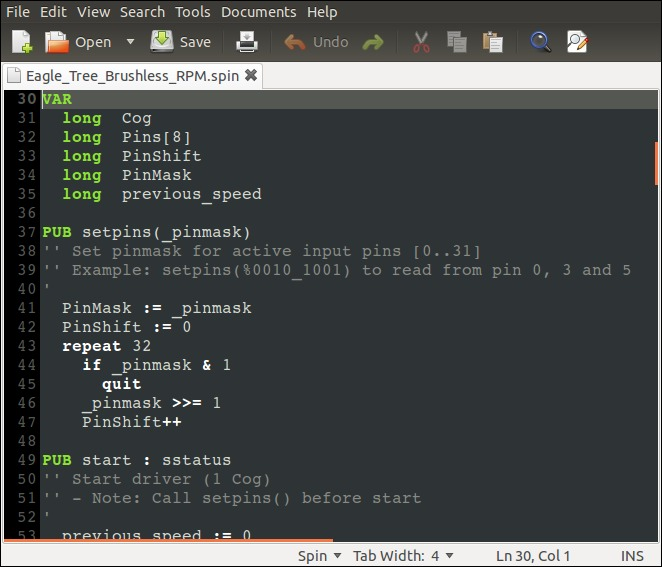
\includegraphics[scale=.4]{gedit_spin_screenshot.jpg}
  \caption{A screenshot of an open Spin file in Gedit showing syntax highlighting.}
\end{figure}  
 
To facilitate the development cycle a simple compilation script was developed. A template form of this script can be found in \\ $/software/spin/tool/bst_-template.sh$. This script will compile the Spin program, and if no errors are found it will attempt to download to the Propeller. If successful it will open picocom (terminal program) on the USB port to listen for data. Using this script while programming dramatically decreases the write-compile-test debug cycle.

%\clearpage %make room for the picture


All code was written in Gedit. Gedit is a simple text editor with a few features built in, including syntax highlighting. For most of the languages in this project, Gedit has provided suitable syntax highlighting. Propeller Spin, however, is not available by default. Syntax highlighting was accomplished by writing a language definition file ($/software/spin/tool/spin.lang$) and placing it in $/usr/share/gtksourceview-3.0/language-specs$. Gedit will then automatically highlight the Spin files.

%%TODO: update the file path typesetting.

All code is compiled with the \texttt{BSTC} compiler. This is available in \cite{campbell09}. This compiler was selected because it is Linux compatible and it has several optimizations over the Parallax provided compiler. In addition, it has a command line interface which makes it easy to integrate into a compilation cycle script. \texttt{BSTC} will also download the compiled code via the USB COM port to the Propeller.

All project files are hosted on the project Git repository, hosted by Google Code at \cite{anzhelka_code}. A Git repository was selected so that all developers would have equal access to the source files, changes would be logged and trackable, issues would be trackable, and so that concurrent work on files  could be easily merged. All project files are open source under the MIT license and can be downloaded freely.

%% S2 S2 S2 S2 S2 S2 S2 S2 S2 S2 S2 S2 S2 S2 S2 S2 S2 S2 S2 S2  
\subsection{Related Documents and Supporting Materials}
TODO
TODO
TODO
TODO
%% S2 S2 S2 S2 S2 S2 S2 S2 S2 S2 S2 S2 S2 S2 S2 S2 S2 S2 S2 S2 

%% S2 S2 S2 S2 S2 S2 S2 S2 S2 S2 S2 S2 S2 S2 S2 S2 S2 S2 S2 S2  
\subsection{Definitions and Acronyms}
\begin{tabular}{l l}
	AT & Anzhelka Terminal \\
	\$ATxxx & Anzhelka Terminal Communication String \\
	BSTC & Brad's Spin Tool Compiler \\
	EEPROM & Electrically Erasable Programmable Read-Only Memory \\
	ESC & Electronics Speed Controller \\
	GUI & Graphical User Interface \\
	IMU & Inertial Measurement Unit \\
	OOP & Object Oriented Programming \\
	PASM & Propeller Assembly \\
	PCB & Printed Circuit Board \\
	PID & Proportional-Integral-Derivative \\
	PWM & Pulse Width Modulation \\
	RAM & Random Access Memory \\
	RISC & Reduced Instruction Set Computer\\
	UART & Universal Asynchronous Receiver /Transmitter (serial) \\
	UAV & Unmanned Aerial Vehicle \\
	WYSIWYG & What You See Is What You Get \\
\end{tabular}
%% S2 S2 S2 S2 S2 S2 S2 S2 S2 S2 S2 S2 S2 S2 S2 S2 S2 S2 S2 S2



%% S1 S1 S1 S1 S1 S1 S1 S1 S1 S1 S1 S1 S1 S1 S1 S1 S1 S1 S1 S1  
\section{Requirements Specifications}
In this section we define the various requirements of the quadrotor platform. The quadrotor must be able to achieve various goals, and since it is a hard real time system the goals must be achieved by a specified deadline.
%% S1 S1 S1 S1 S1 S1 S1 S1 S1 S1 S1 S1 S1 S1 S1 S1 S1 S1 S1 S1  


%% S2 S2 S2 S2 S2 S2 S2 S2 S2 S2 S2 S2 S2 S2 S2 S2 S2 S2 S2 S2  
%\subsection{Guiding Vision}
%Have you ever mounted a camera on to your helmet and rode down a mountainous trail? What about trying to capture yourself while water skiing? Watching the video usually turns out shaky and in one perspective. Would it be nice to be able to see what you did wrong that caused you to fall of your bike? Most of the time you can't see what went wrong. What if you could do all of that while still capturing amazing views?  All this can be accomplished while being as simple as powering on a couple of devices. Simply launch your quadrotor with the press of a button, and get amazing video. This is our vision for the project.
%% S2 S2 S2 S2 S2 S2 S2 S2 S2 S2 S2 S2 S2 S2 S2 S2 S2 S2 S2 S2  

\subsection{Assumptions}
For this project, we assume that the quadrotor frame is rigid and that the propellers are rigid. We assume that the IMU orientation information is correct and without error. We expect the quadrotor to operate in still air, and that it moves slowly through the air.

%% S2 S2 S2 S2 S2 S2 S2 S2 S2 S2 S2 S2 S2 S2 S2 S2 S2 S2 S2 S2  
\subsection{Realistic Constraints}
Every system has constraints and Anzhelka is no exception. The most important constraint is the life of the battery. If each motor consumes 15 amps on average then that is a current drain of 60 amps from the motor battery. Assuming that the battery has 6Ah of energy, then it would be able to power the quadrotor for 10 minutes. Typical flight times for this platform are around 15 minutes, so average current drain is likely less.

The system is also constrained by the maximum acceleration and maximum rotation speed of the propellers. Typically the propeller will not rotate faster than 1200 rpm. This in turn constrains the maximum thrust and torque generated by the motor.

Finally, the system is also constrained by the mass of the vehicle. Since the quadrotor has inertia, to change it's motion requires a greater force from the motors. The motors might not have the power or orientation to change the quadrotor momentum.

%% S2 S2 S2 S2 S2 S2 S2 S2 S2 S2 S2 S2 S2 S2 S2 S2 S2 S2 S2 S2  

%% S2 S2 S2 S2 S2 S2 S2 S2 S2 S2 S2 S2 S2 S2 S2 S2 S2 S2 S2 S2  
\subsection{System Environment and External Interfaces}

To be able to accomplish all of these tasks there are many of interfacing between many different devices. Our main control board must control all 4 ESC's, communicate with the IMU via a serial UART, control servos via PWM signals, monitor the voltage and current of each motor via A2D circuits, and compute the control loop.
%% S2 S2 S2 S2 S2 S2 S2 S2 S2 S2 S2 S2 S2 S2 S2 S2 S2 S2 S2 S2   

%% S2 S2 S2 S2 S2 S2 S2 S2 S2 S2 S2 S2 S2 S2 S2 S2 S2 S2 S2 S2  
\subsection{Industry Standards}
\begin{list}{*}{}
	\item USB
	\item UART
	\item USART
	\item GPS
\end{list}
%% S2 S2 S2 S2 S2 S2 S2 S2 S2 S2 S2 S2 S2 S2 S2 S2 S2 S2 S2 S2  

%% S2 S2 S2 S2 S2 S2 S2 S2 S2 S2 S2 S2 S2 S2 S2 S2 S2 S2 S2 S2  
\subsection{Budget and Cost Analysis}
Unfortunately there was no money that was given to the team in order to support the project. All of the funding has been from the team members' personal accounts. As of this writing, \$3156.24 has been spent on parts for the project. Below is the estimated cost per quadrotor vehicle:
\newpage
\begin{longtable}{l l l l l}
	\textbf{Supplier}		&	\textbf{Name}	&	\textbf{Unit}	&	\textbf{Qty}	&	\textbf{Total}		 \\
	\hline
	Parallax		&	Altimeter	&	\$29.99	&	1	&	\$29.99		 \\
	\hline
	Parallax		&	Propeller Chip QFP	&	\$7.99	&	1	&	\$7.99		 \\
	\hline
	Parallax		&	64KB EEPROM	&	\$1.99	&	1	&	\$1.99		 \\
	\hline
	Parallax		&	5 MHz Crystal	&	\$1.10	&	1	&	\$1.10		 \\
	\hline
	Sparkfun		&	Radio Modem UM96	&	\$44.95	&	2	&	\$89.90		 \\
	\hline
	Hobby King		&	450 Outrunner Motor - Trinigy	&	\$14.04	&	4	&	\$56.16		 \\
	\hline
	Hobby King		&	30A ESC	&	\$5.99	&	4	&	\$23.96		 \\
	\hline
	Hobby King		&	3S 30C 1000mAh Battery	&	\$8.99	&	1	&	\$8.99		 \\
	\hline
	Hobby King		&	3S 30C 8000mAh Battery	&	\$44.11	&	1	&	\$44.11		 \\
	\hline
	Hobby King		&	Deans XT Plugs (10 pairs)	&	\$3.08	&	2	&	\$6.16		 \\
	\hline
	Hobby King		&	12 AWG 1 meter wire Black	&	\$2.49	&	3	&	\$7.47		 \\
	\hline
	Hobby King		&	12 AWG 1 meter wire Red	&	\$2.49	&	3	&	\$7.47		 \\
	\hline
	McMaster-Carr	&	5/8" Aluminum Tubing 6'	&	\$16.38	&	1	&	\$16.38		 \\
	\hline
	McMaster-Carr	&	3/32" Delrin 24"x48"	&	\$70.67	&	1	&	\$70.67		 \\
	\hline
	McMaster-Carr	&	1/4" Delrin 12"x12"	&	\$27.87	&	1	&	\$27.87		 \\
	\hline
	McMaster-Carr	&	4-40 5/8" Standoff	&	\$0.46	&	12	&	\$5.52		 \\
	\hline
	DIY Drones		&	Propellers 10x4.5 1 push 1 pull	&	\$6.00	&	2	&	\$12.00		 \\
	\hline
	Pololu			&	CHR-UM6-LT IMU Sensor	&	\$149.99	&	1	&	\$149.99		 \\
	\hline
	Anzhelka		&	Power control board	&	\$166.60	&	1	&	\$166.60		 \\
	\hline
	Tower Hobbies	&	Eagle Tree RPM sensor	&	\$13.79	&	4	&	\$55.16		 \\
	\hline
	\textbf{Total}	&		&		&		&	\textbf{\$789.48}
\end{longtable}



%% S2 S2 S2 S2 S2 S2 S2 S2 S2 S2 S2 S2 S2 S2 S2 S2 S2 S2 S2 S2

%% S2 S2 S2 S2 S2 S2 S2 S2 S2 S2 S2 S2 S2 S2 S2 S2 S2 S2 S2 S2  
\subsection{Safety}

When dealing with any robotic system one must take extreme cautions in order to ensure the safety of everyone. Autonomous systems are particularly dangerous because there is human behind the controls of the system and can become unpredictable in the event of a system failure. 

Several precautions are enacted to decrease the likelyhood of accidents. During frame construction the team uses fasteners, washers, and nuts that are of suitable specification. All threaded components are secured using blue Loctite to ensure that nothing will loosen on its own. Whenever motors are spinning safety glasses are required. This provides protection in the event that a propeller has a failure and is detached/released from the motor.
%% S2 S2 S2 S2 S2 S2 S2 S2 S2 S2 S2 S2 S2 S2 S2 S2 S2 S2 S2 S2  

%% S2 S2 S2 S2 S2 S2 S2 S2 S2 S2 S2 S2 S2 S2 S2 S2 S2 S2 S2 S2  
\subsection{Documentation}
Throught the design, build and testing phase of this project we have been documenting any and all information of interesting on the Anzhelka Blog. (\cite{anzhelka_blog})
%% S2 S2 S2 S2 S2 S2 S2 S2 S2 S2 S2 S2 S2 S2 S2 S2 S2 S2 S2 S2  

%% S2 S2 S2 S2 S2 S2 S2 S2 S2 S2 S2 S2 S2 S2 S2 S2 S2 S2 S2 S2  
\subsection{Understanding of Professional and Ethical Responsibility}
Unmanned aerial vehicles(UAVs) are a very controversial current topic. The Anzhelka project is part of a subset of UAVs; namely, vertical take and and landing (VTOL). UAVs can assist in surveillance, inspect structures, creating aerial photographs, rescuers in a disaster situation, transporting goods, and many other situations. However, UAVs can also reduce privacy and security of individuals.
%% S2 S2 S2 S2 S2 S2 S2 S2 S2 S2 S2 S2 S2 S2 S2 S2 S2 S2 S2 S2  

%% S2 S2 S2 S2 S2 S2 S2 S2 S2 S2 S2 S2 S2 S2 S2 S2 S2 S2 S2 S2  
\subsection{Global, Economic, Environmental and Societal Impact}
The Anzhelka project could potentially have a large global impact. Our project can change the way things are monitored. With a quadrotor you can monitor a target from a distance without having to move around to stay at the same altitude. Quadrotors also have a greater payload capacity over helicopters because they are much lighter by design.
%% S2 S2 S2 S2 S2 S2 S2 S2 S2 S2 S2 S2 S2 S2 S2 S2 S2 S2 S2 S2  

%% S2 S2 S2 S2 S2 S2 S2 S2 S2 S2 S2 S2 S2 S2 S2 S2 S2 S2 S2 S2  
\subsection{Contemporaray Engineering Issues}
\begin{list}{*}{}
	\item Power Management
	\item Motor Control and Monitoring
	\item Weight
	\item Size
	\item Safety
	\item PCB design
\end{list}
%% S2 S2 S2 S2 S2 S2 S2 S2 S2 S2 S2 S2 S2 S2 S2 S2 S2 S2 S2 S2  

%% S2 S2 S2 S2 S2 S2 S2 S2 S2 S2 S2 S2 S2 S2 S2 S2 S2 S2 S2 S2  
\subsection{Lifelong Learning}
The Anzhelka Project is a living breathing project. It has the possiablity to be expanded in many different ways. During this project the team had discovered lots of flaws in off the self hobbiest electronics. The IMU that was used did not provide the adequate data that it said it was able to provide. The motor drivers do not have feed back to the controller to let it know RPM, Voltage, or Current. These are just some of the things that were encountered and are planned to be changed by the Anzhelka team.
%% S2 S2 S2 S2 S2 S2 S2 S2 S2 S2 S2 S2 S2 S2 S2 S2 S2 S2 S2 S2  

%% S2 S2 S2 S2 S2 S2 S2 S2 S2 S2 S2 S2 S2 S2 S2 S2 S2 S2 S2 S2  
\subsection{Importance of Team Work}
Being able to work in a team is both a skill and a challenge. Working on a project in a group helps you split up the work load and possibly get more work done in less time, however being able to work together with others on the project could present a greater challenge than the project itself. 

This was a foreseen challenge and the team set up a Git repository for all code, data, images, and presentations. There was also an official blog set up where we could go in great detail on what we were working on and what we had yet to complete. With these two resources set up and with the help of keeping an open schedule the team has been able to successfully coordinate and maximize productivity.
%% S2 S2 S2 S2 S2 S2 S2 S2 S2 S2 S2 S2 S2 S2 S2 S2 S2 S2 S2 S2



%clearpage %make room for the picture
%% S1 S1 S1 S1 S1 S1 S1 S1 S1 S1 S1 S1 S1 S1 S1 S1 S1 S1 S1 S1  
\section{High Level Design}
The system is fairly simple. The general system architecture consists of the central Propeller microcontroller interfacing with a number of different devices. Both hardware and software mimic this layout, which is shown below.

%\clearpage %make room for the picture
\begin{figure}[h!]
  \centering
	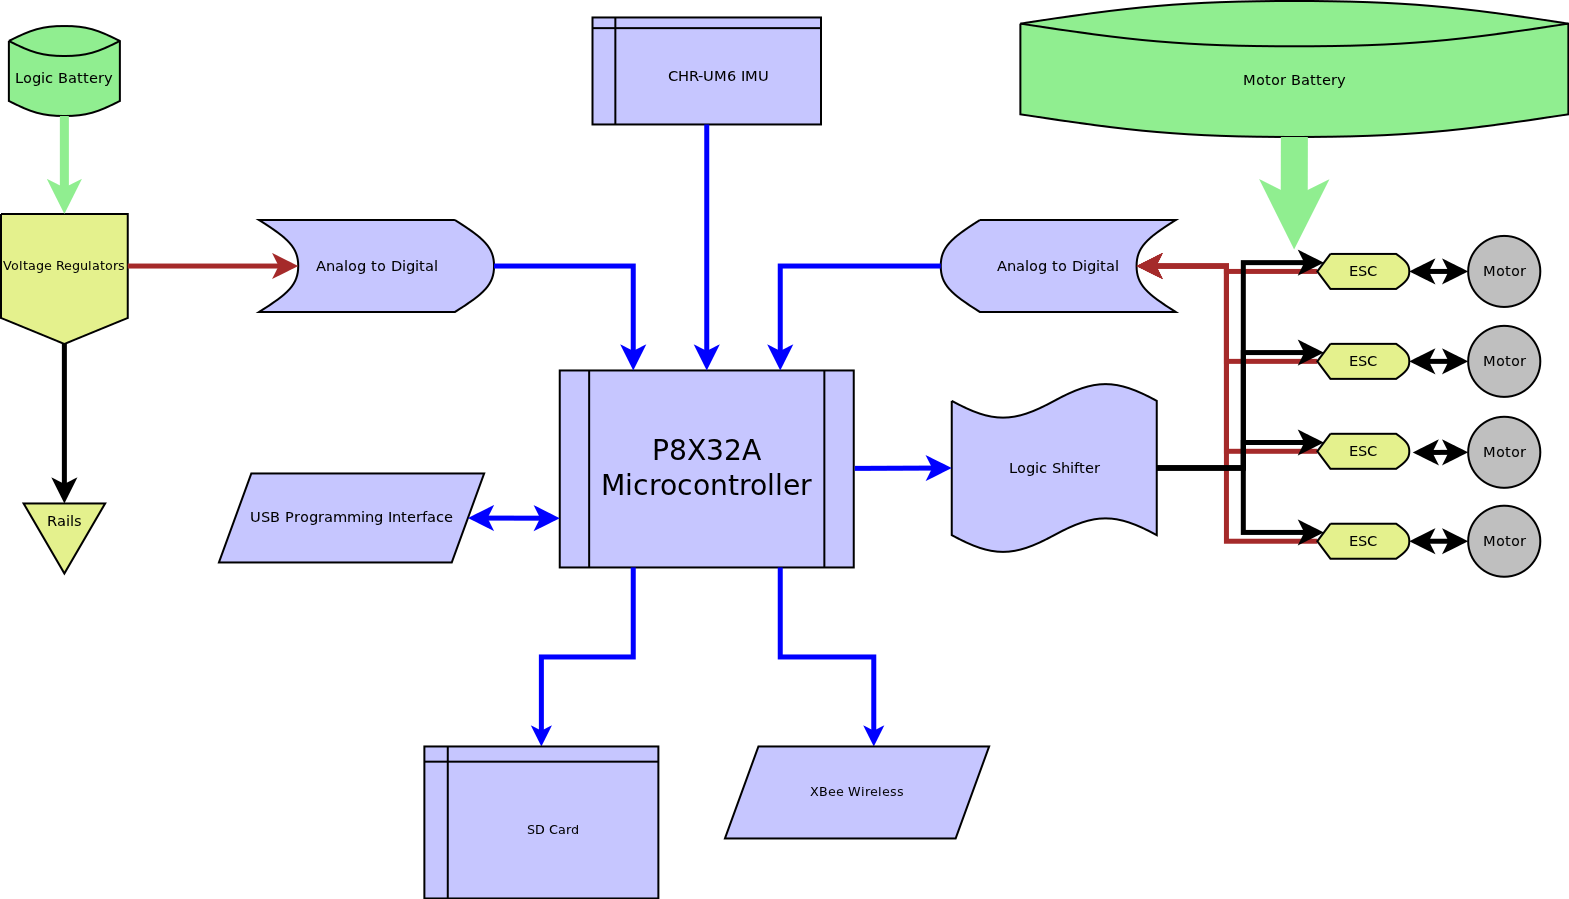
\includegraphics[scale=.22]{system_architecture.png}
  \caption{The layout of the devices in the system at a hardware level.}
\end{figure}  

%% S1 S1 S1 S1 S1 S1 S1 S1 S1 S1 S1 S1 S1 S1 S1 S1 S1 S1 S1 S1

%% S2 S2 S2 S2 S2 S2 S2 S2 S2 S2 S2 S2 S2 S2 S2 S2 S2 S2 S2 S2  
%\subsection{Experiment Design}
%% S2 S2 S2 S2 S2 S2 S2 S2 S2 S2 S2 S2 S2 S2 S2 S2 S2 S2 S2 S2  

%% S2 S2 S2 S2 S2 S2 S2 S2 S2 S2 S2 S2 S2 S2 S2 S2 S2 S2 S2 S2  
%\subsection{Experiment Results and Feasibility}
%% S2 S2 S2 S2 S2 S2 S2 S2 S2 S2 S2 S2 S2 S2 S2 S2 S2 S2 S2 S2  

%% S1 S1 S1 S1 S1 S1 S1 S1 S1 S1 S1 S1 S1 S1 S1 S1 S1 S1 S1 S1  
\section{Low Level Design}
This section describes the quadrotor's low level design.
%% S2 S2 S2 S2 S2 S2 S2 S2 S2 S2 S2 S2 S2 S2 S2 S2 S2 S2 S2 S2  
\subsection{Propeller}
For this project we selected the Parallax Propeller as our main embedded processor. This chip has several unique features that make it well suited to the real time requirments of quadrotoor flight. The Propeller is relatively inexpensive as well: \$8 per chip, plus approximately \$2 for support components.

%% S3 S3 S3 S3 S3 S3 S3 S3 S3 S3 S3 S3 S3 S3 S3 S3 S3 S3 S3 S3  
\subsubsection{Architecture}

The Propeller microcontroller has a unique architecture. The Propeller is a microcontroller is a 8 core 32 bit RISC processor. For this project the Propeller has been overclocked from the default 80MHz to 100MHz. This additional speed facilitates more complex computations without sacrificing output rate. Each core, called a COG, is identical with equal access to all chip resources. The Propeller has a central RAM area called the HUB which is COG accessible in a round robin fashion.

%\clearpage %make room for the picture
\begin{figure}[h!]
  \centering
	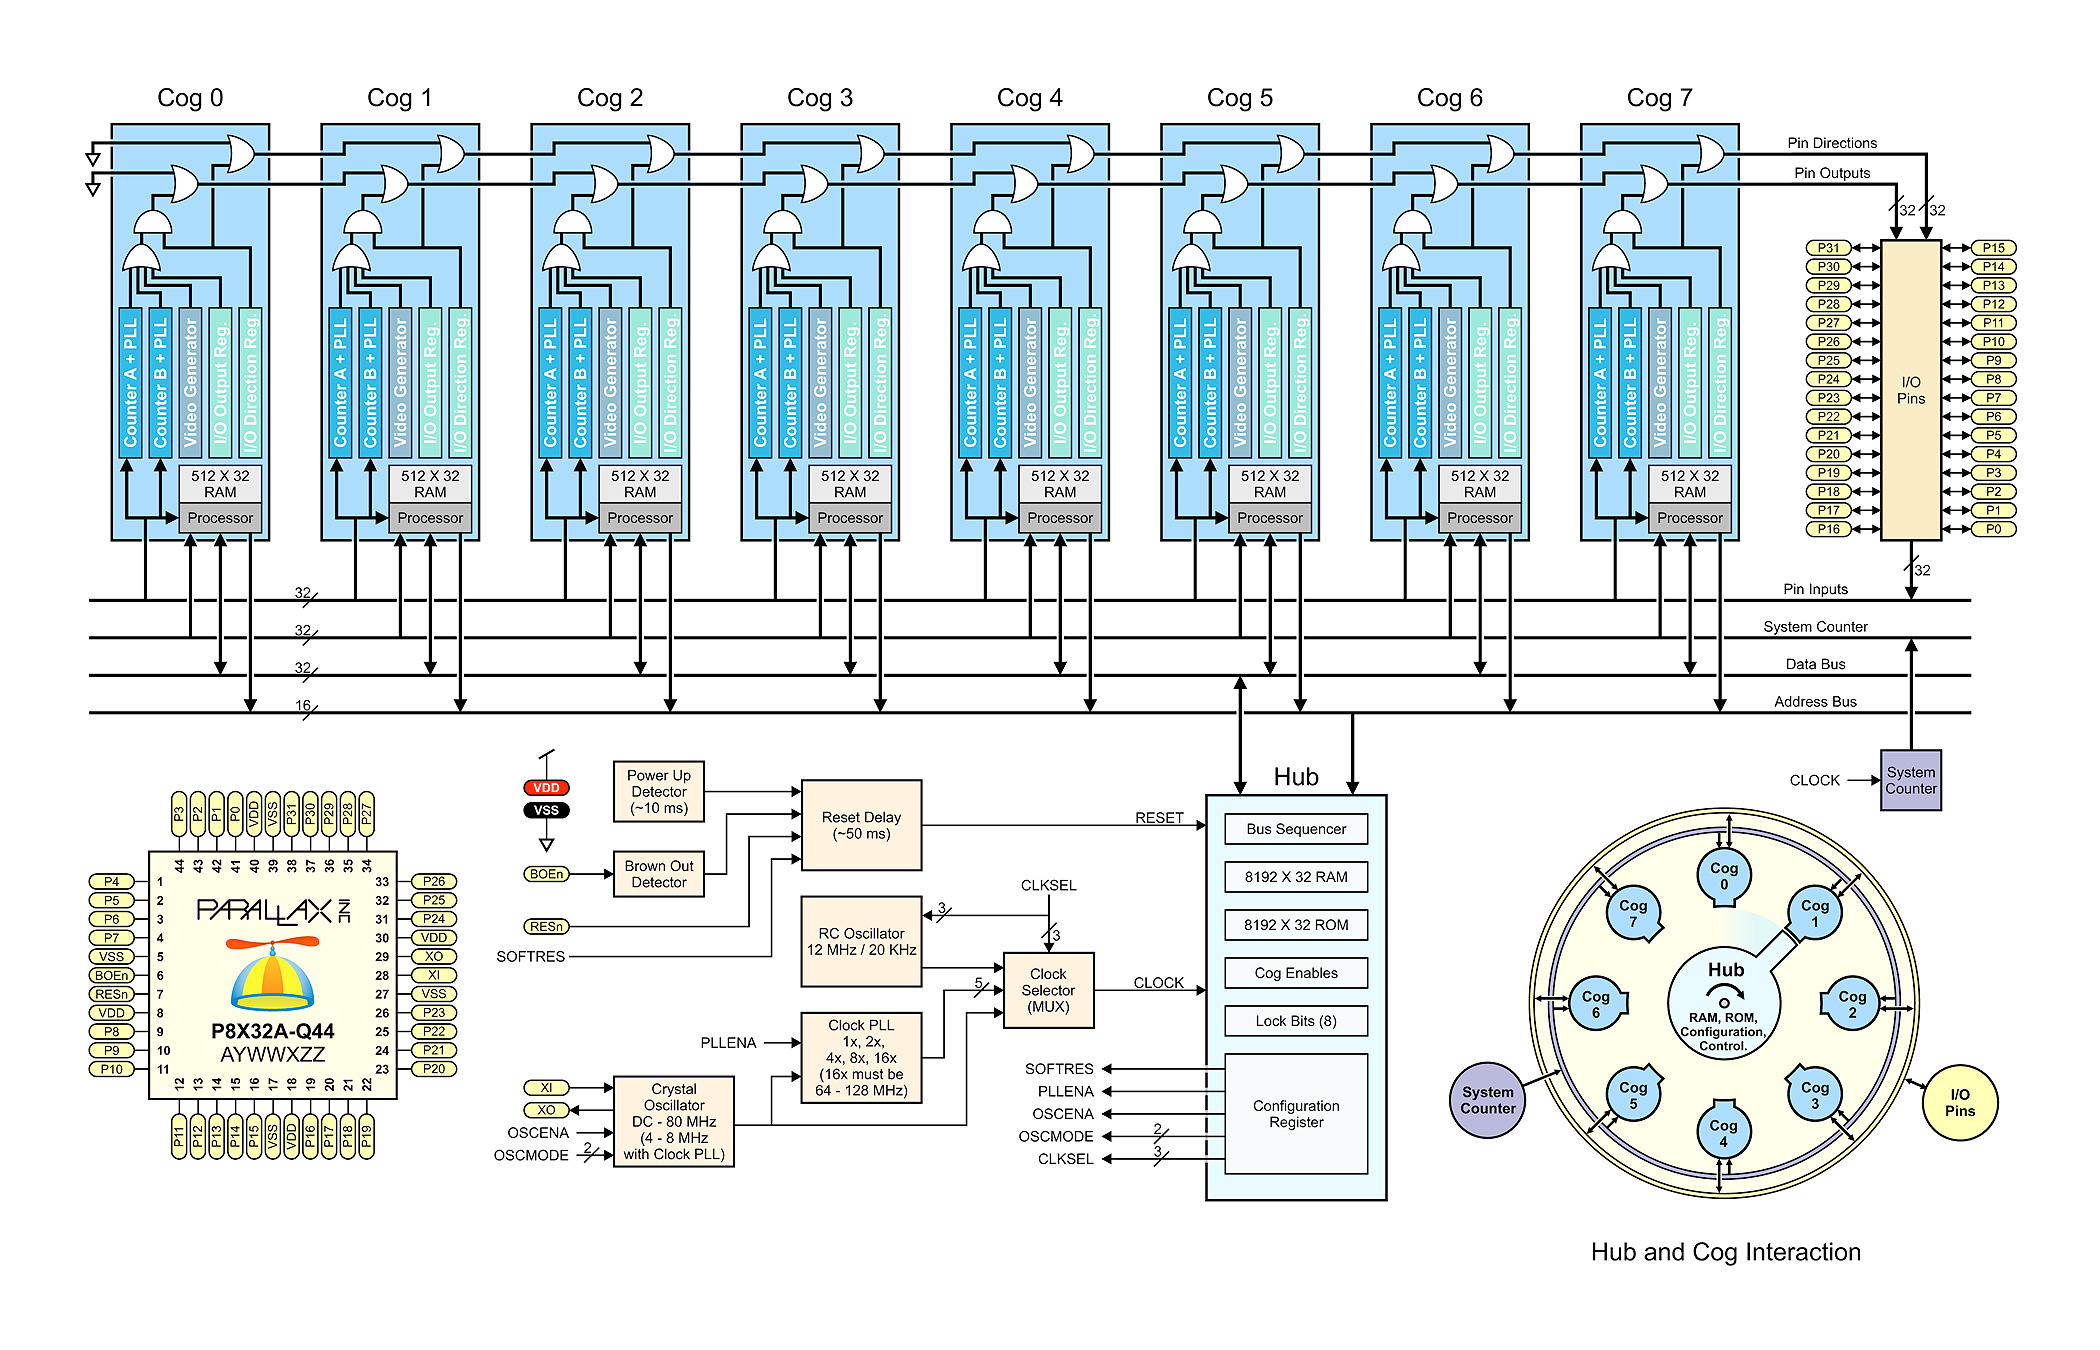
\includegraphics[scale=.17]{PropellerArchitecture.jpg}
  \caption{The functional architecture of the Parallax Propeller (courtesy of Parallax).}
\end{figure}  

The Propeller is distinctly different from most other microcontrollers by it's lack of built in hardware. The Propeller does not have any hardware level serial ports, analog to digital or digital to analog ports, or any pulse width modulation ports. Instead, the Propeller is designed to be able to use software for these common interfaces. This is typically done through what is known as “bit banging.” The only exception is the built in video generation hardware that assists in creating NSTC, PAL, or VGA signals. To make development easier for the programmer, Parallax hosts a source code website that provides code for common tasks such as serial or PWM.

The Propeller has two built in languages: a high level language called Spin and the assembly language called PASM. PASM is executed directly by a COG. Spin is executed by a built in PASM Spin interpreter that can be dynamically loaded into one or more COGs. Other high level languages available for the Propeller generally operate in a similar manner to Spin. This project uses Spin and PASM exclusively.

The Propeller has three different memory locations: 2KB of COG RAM, 32KB of HUB RAM, and external 64KB of I2C EEPROM. Upon startup, the Propeller copies the contents of the EEPROM to HUB RAM, loads a Spin interpreter into COG 0, and begins execution.  Any PASM code, including the Spin interpreter, must fit in 496 instructions or less in order to fit into the COG RAM. The Propeller does not have provisions for fetching PASM instructions from other locations besides COG RAM. For Spin code the compiled interpretable bytes are stored in the HUB RAM, and are fetched and decoded by the Spin interpreter.
%% S3 S3 S3 S3 S3 S3 S3 S3 S3 S3 S3 S3 S3 S3 S3 S3 S3 S3 S3 S3  

%% S3 S3 S3 S3 S3 S3 S3 S3 S3 S3 S3 S3 S3 S3 S3 S3 S3 S3 S3 S3  
\subsubsection{Programming}

The Propeller is programmed in PASM and a high level language called Spin. In general, PASM is used when speed is required. At 100MHz, the Propeller can execute 25,000,000 assembly instructions each second (each instruction takes 40ns). By contrast, the interpreted Spin language is about 100x slower. Because of this contrast Spin is used where ease of programming is important, and PASM is used where speed is important.

Spin is officially called an object oriented programming language, but there are some subtle differences compared to mainstream object oriented terminology. Spin OOP is used to organize code into logical blocks much like an import statement in C++ or Python. Spin objects do not use techniques such as class instances, inheritance, or subtype polymorphism. A Spin object is used to group related functions together into a unit that can be included in multiple Spin programs. 

Typically, Spin objects are used for interfacing with external devices. For example, a typical Spin program might have an object for serial communication, an object for VGA signal generation, and an object for I2C communication. The Parallax Object Exchange (\cite{parallaxobjectexchange}) hosts Parallax written objects and community written objects under the open source MIT licence.

Spin syntax is very similar to Python. To denote a new scope Spin uses indentation instead of curly braces {} (familiar to C/C++ and Java programmers). Spin code is divided into blocks: CON (constant), VAR (variable), OBJ (object), DAT (data), PUB (public function), and PRI (private function). Most typical programming constructs are a part of the Spin language: conditional IF statements, FOR loops (called REPEAT), boolean conditions, and so on.

All variables in the Propeller are integers. Variables are typically 32 bit signed integers called longs, but in Spin it is possible to create 16 bit or 8 bit sized variables as well (called words and bytes, respectively). Global variables are declared in the VAR block, and global constants are declared in the CON block. PRI and PUB functions can declare local variables, along with function parameters. 
%% S3 S3 S3 S3 S3 S3 S3 S3 S3 S3 S3 S3 S3 S3 S3 S3 S3 S3 S3 S3  
%% S2 S2 S2 S2 S2 S2 S2 S2 S2 S2 S2 S2 S2 S2 S2 S2 S2 S2 S2 S2  

\subsection{Control Loop Frequency} \label{subsec:codeperformanceestimation}

For our software, the critical portion is the main control loop that keeps the quadrotor flying at the desired attitude (roll, pitch, yaw) and altitude. It is essential that this control loop operates fast enough to respond to disturbances. From our research into what other quadrotor groups have done we have found that 50Hz to 75Hz is sufficient for flying. So for our project we need to analyze our system and determine if we can achieve the desired rate.

The first component to consider is the inertial measurement unit (IMU). The IMU that we have selected is the CHR-UM6-LT IMU. From the datasheet, it can output at up to 300 Hz. On the output we have the ESCs that control the motors. These expect a control pulse every 20ms, so that is on update rate of 50Hz. Most stock components can run with a slightly faster update rate, and we can select ESCs that are designed for a faster rate. In any case, we have guaranteed support for 50Hz updates with the hardware we have.

Now we need to consider the software control loop. We've broken the math into three blocks: attitude control, altitude control, and motor control. The equations can be found in the Anzhelka mathematics document \cite{anzhelka_math}. The attitude control block and altitude control block can be done in parallel, and their output fed into the motor control block. We will be writing the code in Propeller Assembly using the Float32 floating point library (\cite{float32}).

The Float32 documentation includes timings and space requirements for each of the mathematical functions. If we count the operations required for each block we can then calculate an estimate of running time and space.

First, we have to count up all of the operations so we know how much math we have to do:


\begin{longtable}{l l l l l l l l l l l l l}
Quantity&	
\begin{sideways}+\end{sideways}	&	
\begin{sideways}-\end{sideways}	&	
\begin{sideways}*\end{sideways}	&	
\begin{sideways}/\end{sideways}	&	
\begin{sideways}cos\end{sideways}	&	
\begin{sideways}sin\end{sideways}	&	
\begin{sideways}asin\end{sideways}	&	
\begin{sideways}acos\end{sideways}	&	
\begin{sideways}atan2\end{sideways}	&	
\begin{sideways}sqrt\end{sideways}	&	
\begin{sideways}quat*\end{sideways}	&	
\begin{sideways}Sum\end{sideways}\\
	\hline
Moment	&	1	&	6	&	20	&	11	&	3	&	4	&	0	&	2	&	2	&	0	&	3	&	52 \\
	\hline
Altitude &	3	&	1	&	4	&	1	&	0	&	0	&	0	&	0	&	0	&	0	&	2	&	11	 \\
	\hline
Motor Speed	&	14	&	10	&	18	&	10	&	0	&	0	&	0	&	0	&	0	&	4	&	0	&	56		 \\
	\hline
	Sum	&	18	&	17	&	42	&	22	&	3	&	4	&	0	&	2	&	2	&	4	&	5	&	119	\\
\end{longtable}

Our control loop has 119 mathematical operations. The number sounds small, but it is slightly misleading. In the next table we see that the time to execute an addition or multiplication is much less than it is to calculate arcsin or arccos. For quaternion multiplication we assume that one multiply has 6 floating point additions, 6 floating point subtractions, and 16 floating point multiplies. This follows from the quaternion multiplication formula. In summary, since we have the number of each operation, we can calculate the total times:

\begin{longtable}{l l l l l l l l l l l l l l l l l l l }
\textbf{Operator}&	
\begin{sideways}+\end{sideways}	&	
\begin{sideways}-\end{sideways}	&	
\begin{sideways}*\end{sideways}	&	
\begin{sideways}/\end{sideways}	&	
\begin{sideways}cos\end{sideways}	&	
\begin{sideways}sin\end{sideways}	&	
\begin{sideways}asin\end{sideways}	&	
\begin{sideways}acos\end{sideways}	&	
\begin{sideways}atan2\end{sideways}	&	
\begin{sideways}sqrt\end{sideways}	&	
\begin{sideways}quat*\end{sideways}	&	
\begin{sideways}Sum ($\mu s$)\end{sideways} \\
	\hline
Unit Time&	3.7	&	3.8	&	8.4	&	10	&	78	&	74	&	261	&	265	&	117	&	173	&	225	&\\
	\hline
Moment	&	3	&	23	&	168	&	116&	234	&	298	&	0	&	530	&	234	&	0	&	675	&	2283 \\
	\hline
Altitude	&	11	&	3	&	33	&	10	&	0	&	0	&	0	&	0	&	0	&	0	&	450	&	 \sout{\textit{509}} \\
	\hline
Motor	&	52	&	38	&	151	&	105	&	0	&	0	&	0	&	0	&	0	&	694	&	0	&	1042\\
	\hline
Sum	&	67	&	65	&	352	&	232	&	234	&	298	&	0	&	530	&	234	&	694	&	1125	&	\textbf{3325}\\	
\end{longtable}


Our estimates show that we can have an inner control loop of 260Hz, and if we parallelize the moment and altitude calculations as shown above then we can get about 40Hz faster for a control loop frequency of 300 Hz. Also of interest is that the quadrotor control loop has a response time of 3.3 milliseconds. For reference, the average human reaction time is roughly 200 milliseconds (\cite{human_reaction_time}).

Finally, we are interested in code size. The floating point library has a number of required support functions that do things such as convert to and from floating point, compare floats, and so on that require space. We also assume that 4 longs on average are used to setup each operation. This gives totals of
\begin{longtable}{l l}
	\textbf{Block} & \textbf{Longs} \\
	Moment		& 552 \\
	Altitude	& 275 \\
	Motors		& 468 \\
\end{longtable}

So, if we were to do each instruction in sequence then it would take approximately 850 longs (sum without duplicates). Unfortunately, a Propeller cog only has enough memory for 496 longs. If we break it into sections then the altitude and motor calculations will fit into a single cog, but the moment block is too big. Some optimizations will probably be able to reduce the size to fit.

All in all, the code performance estimates are looking very promising. We should be able to achieve 100Hz update rates and the use of only two cogs without too much trouble.

%% S2 S2 S2 S2 S2 S2 S2 S2 S2 S2 S2 S2 S2 S2 S2 S2 S2 S2 S2 S2 
\subsection{Other Software Notes}
The other software in this project is standard. This project uses a Phython GUI and a shell script for program compilation.


%% S2 S2 S2 S2 S2 S2 S2 S2 S2 S2 S2 S2 S2 S2 S2 S2 S2 S2 S2 S2  

%% S1 S1 S1 S1 S1 S1 S1 S1 S1 S1 S1 S1 S1 S1 S1 S1 S1 S1 S1 S1  
  

%% S1 S1 S1 S1 S1 S1 S1 S1 S1 S1 S1 S1 S1 S1 S1 S1 S1 S1 S1 S1  
\section{Quadrotor Prototype Construction}
A quadrotor to the specifications is being constructed for this project.
%\textcolor{green}{\bf Given the relatively short duration of the class, completion of the project may not be possible; however, you must do your best to produce a working prototype that implements the most important core functionality of the system you have envisions. If graphical output is not possible, create some screen mock-ups on your own.}
%% S1 S1 S1 S1 S1 S1 S1 S1 S1 S1 S1 S1 S1 S1 S1 S1 S1 S1 S1 S1  

%% S2 S2 S2 S2 S2 S2 S2 S2 S2 S2 S2 S2 S2 S2 S2 S2 S2 S2 S2 S2  
%\subsection{Intermediate Project Reports}
%\textcolor{green}{\bf Intermediate Project Reports—Document your progress. Both intermediate ! ! ! project reports should describe your progress toward the construction of the overall prototype. This section should include two brief summaries that document your project at the time of the intermediate demonstrations.} \\ \\
%\textcolor{red}{\bf Not required because these were admitted.}
%% S2 S2 S2 S2 S2 S2 S2 S2 S2 S2 S2 S2 S2 S2 S2 S2 S2 S2 S2 S2  

%% S2 S2 S2 S2 S2 S2 S2 S2 S2 S2 S2 S2 S2 S2 S2 S2 S2 S2 S2 S2  
\subsection{Hardware}
At this point in the project, we have developed four main areas of hardware: the quadrotor frame, the motors and propellers used, the power board PCB, and the thrust torque test stand. These components are, roughly, what will be used for the rest of the project and are relatively static. 

\begin{center}
{\bf Frame Dimensions without rotors attached.} (longways) \\
28 1/4 inches (718 mm) X 28 1/4 inches (718 mm) X 4 5/8 inches (117mm)
\\ \bigskip
{\bf Frame Dimensions with rotors attached.} (longways) \\
36 1/4 inches (921 mm) X 36 1/4 inches (921 mm) X 6 3/8 inches (161mm)
\end{center}

\begin{longtable}{l l}
	\textbf{Item} & \textbf{Mass(Grams)} \\
	Frame			& 450g \\
	Each propeller	& 8g \\
	Motor (black)		& 85g \\
	Motor (red)		& 90g \\
	ESC (black)		& 20g \\
	ESC (red)		& 25g \\
	5000MAH Battery	& 410g \\
	8000MAH Battery	& 650g \\
\end{longtable}

%% S2 S2 S2 S2 S2 S2 S2 S2 S2 S2 S2 S2 S2 S2 S2 S2 S2 S2 S2 S2  

%% S3 S3 S3 S3 S3 S3 S3 S3 S3 S3 S3 S3 S3 S3 S3 S3 S3 S3 S3 S3
\subsubsection{Frame}
The quadrotor frame that we are using for this project is the open source Elev-8 frame from Parallax (\cite{elev8_frame})The resin plates are constructed out of a material called Delin\textregistered\cite{dupontdelin} made by DuPont\texttrademark. We had this material laser cut for us by a W9GFO from the Parallax forums. The booms of the Frame are made out of 5/8" thin wall aluminium tubing.

For the screws we are using hex pan head and hex socket cap screws. These screws are very common in the industrial supply industry. For all of the screws we are using blue LocTite or a nylon locknut to ensure that the screws do not loosen from their secured position. Lockwashers are not used due to being completely ineffective and, in fact, worse than nothing at all (\cite{vibration_loose}).

Diagrams for the frame components have been included in the appendices, and are also available at \cite{anzhelka_code}.
%% S3 S3 S3 S3 S3 S3 S3 S3 S3 S3 S3 S3 S3 S3 S3 S3 S3 S3 S3 S3

%% S3 S3 S3 S3 S3 S3 S3 S3 S3 S3 S3 S3 S3 S3 S3 S3 S3 S3 S3 S3
\subsubsection{Motors/Propellers}

Since neither one of the team members has any experience with quadrotors, we have selected two different motors for the testing of our platform. To match with these two motors we picked out two different brands of ESCs in order to determine which would would be best with the platform.

We also decided on a 10 inch rotor with a 4.5 degree pitch. We decided on 10 inches because it gave us plenty of clearance between the rotors and should not produce turbulences between each other. As for pitch, if you want a very stable take off and landing of the quadrotor you would go with less of a pitch, however if you want to be able to translate rather quickly you want more of a pitch. Every fixed pitch propeller is designed for maximum efficiency at a certain free air stream velocity through the blades. Hovering (ie, no free air stream velocity) is most efficient at very small pitches (\cite{propeller_pitch}).
\\
\begin{figure}[h!]
  \centering
	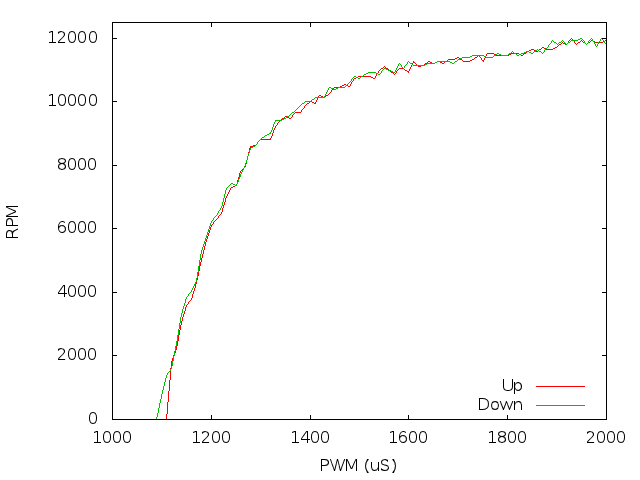
\includegraphics[scale=.40]{pwm_vs_rpm.png}
  \caption{PWM vs RPM under no load. They are nearly the same on the PWM up and down.}
\end{figure}  
\\
\begin{figure}[h!]
  \centering
	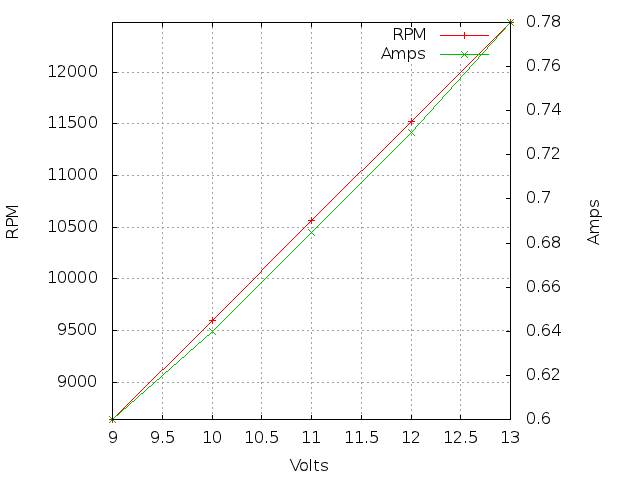
\includegraphics[scale=.40]{volts_vs_rpm.png}
  \caption{Volts vs RPM under no load. As you can see that the current is linear with the voltage.}
\end{figure}  

%% S3 S3 S3 S3 S3 S3 S3 S3 S3 S3 S3 S3 S3 S3 S3 S3 S3 S3 S3 S3
\newpage
%% S3 S3 S3 S3 S3 S3 S3 S3 S3 S3 S3 S3 S3 S3 S3 S3 S3 S3 S3 S3
\subsubsection{Power Board PCB}
For this project we developed a custom circuit board to power the quadrotor. This PCB has all the hardware on it to facilitate a number of features:
\begin{list}{*}{}
	\item Propeller microcontroller, overclockable
	\item Switching regulators for the logic voltages
	\item Power distribution for motor ESCs
	\item Current and voltage sensing for all motors
	\item Level shifting for 5v interfacing
	\item 8 free channel of ADC
	\item 8 free servo channels
	\item I/O headers for I2C, IMU, SD card, and XBee
	\item Mounting holes for BoE formfactor, quickstart, SD card, and IMU
\end{list}

PCBs are very difficult in the ways of being able to produce something that will be small enough to fit on your platform and large enough for you to solder the components onto. The PCB design for the prototype took over a month to layout and design. Even though this may seem like a long time, it is not excessive when dealing with many new components.
%\clearpage %make room for the picture
\begin{figure}[h!]
  \centering
	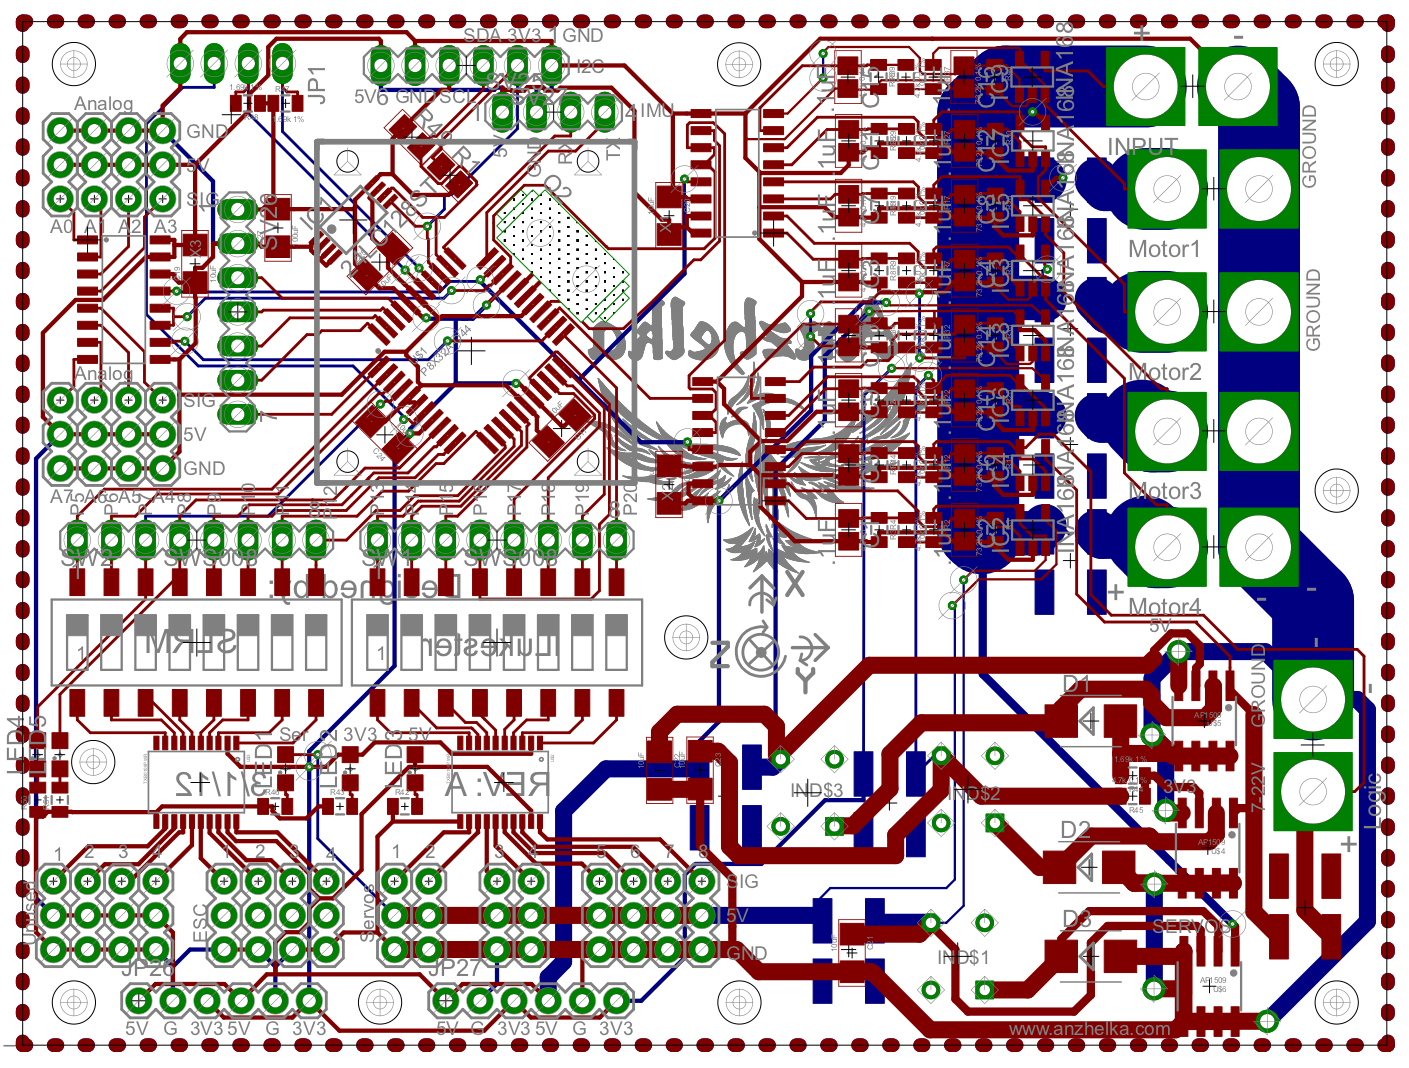
\includegraphics[scale=.23]{revA_both.png}
  \caption{The developed Power Board, REV A. This figure shows both sides of the PCB, along with the silkscreen.}
\end{figure}  
Once the board was designed and ready for production a fabrication house had to be selected. Choosing a fabrication house in the United States provides for a very fast turn around time, but at a much larger cost. Choosing one in China provides for a much cheaper product, but at a slower turn around time. The fabrication house in China that we selected (iTeadStudio) took nearly a month for a full turn around. This is not typical, but was certainly unfortunate.

%\clearpage %make room for the picture
\begin{figure}[h!]
  \centering
	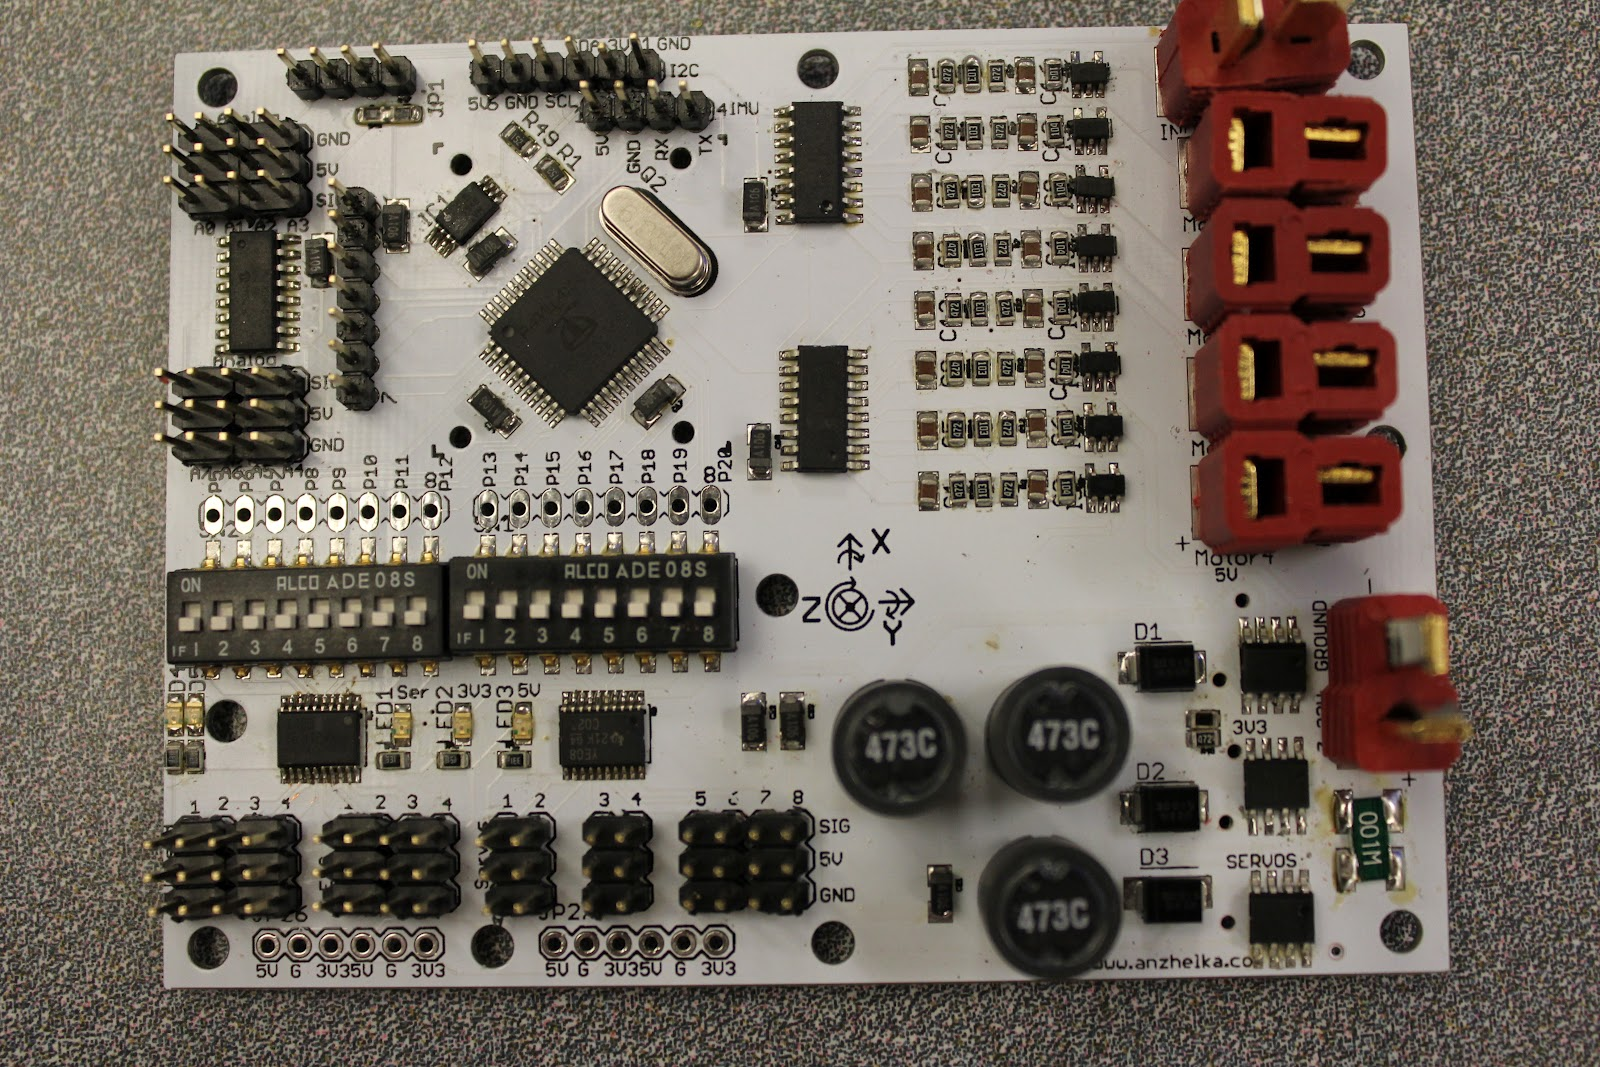
\includegraphics[scale=.2]{populated_pcb_revA.JPG}
  \caption{The finished PCB, populated with components. The Propeller is the rotated chip in the upper left. The red connectors are the Deans plugs for high current connections. On the bottom left are the 3.3v to 5v level shifters.}
\end{figure}  

%% S3 S3 S3 S3 S3 S3 S3 S3 S3 S3 S3 S3 S3 S3 S3 S3 S3 S3 S3 S3

\subsubsection{Thrust/Torque Test Stand Construction}
The thrust/torque test stand was constructed out of wood and metal. Everything was hand crafted. A few components needed machining, and those were done in a machine shop. We developed the test stand from scratch with very little prior work to base the project on. The axles are all supported ball bearings to reduce friction to negligable amounts.

\begin{figure}[ht]
\centering
\subfigure[The thrust/torque test stand.]{
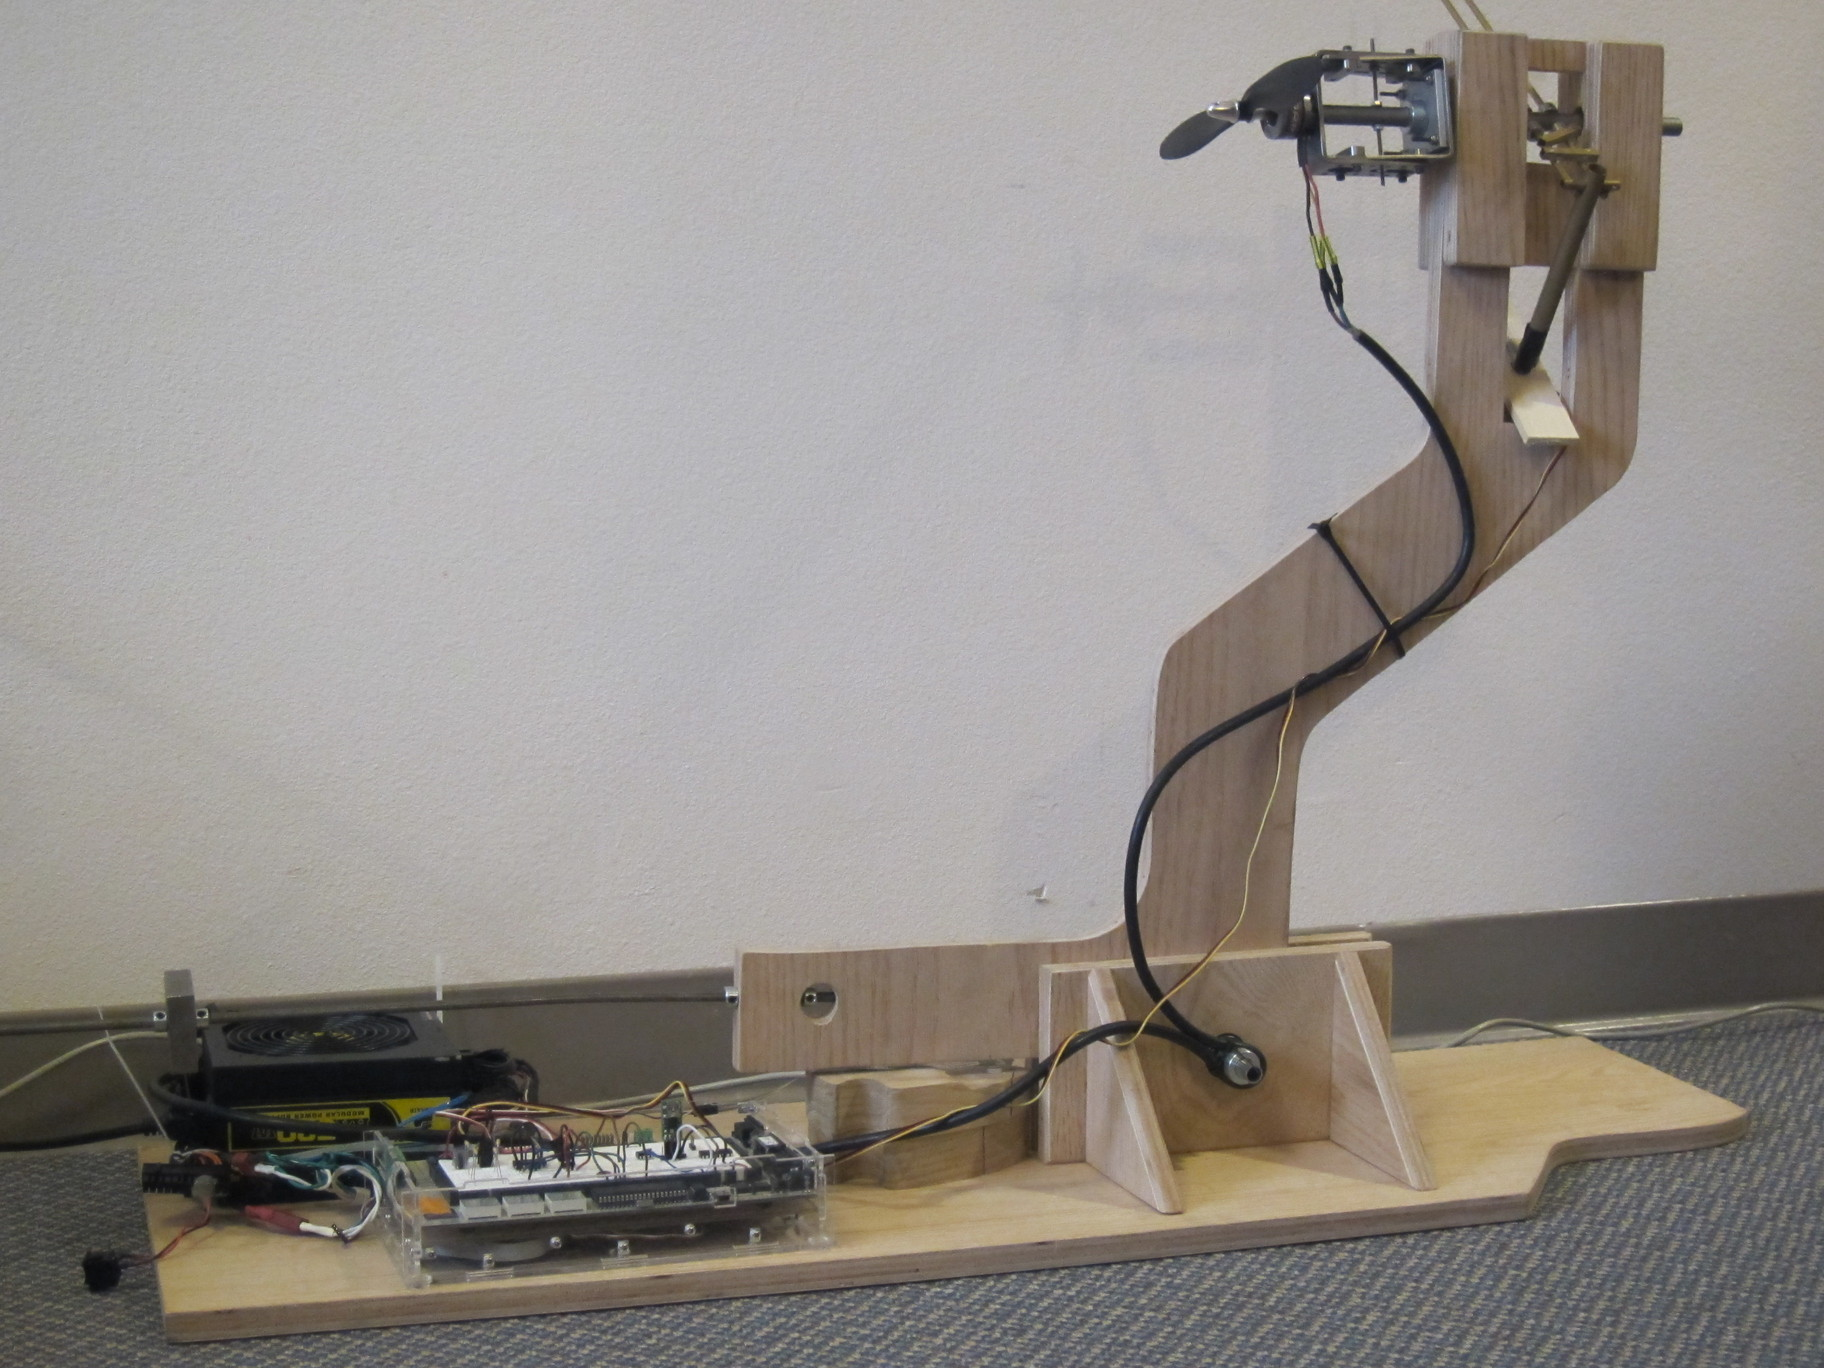
\includegraphics[scale=.22]{thrust_torque_stand_overview.JPG}
}
\subfigure[The motor mounting is on the left and torque measurement arm is the bronze piece on the right.]{
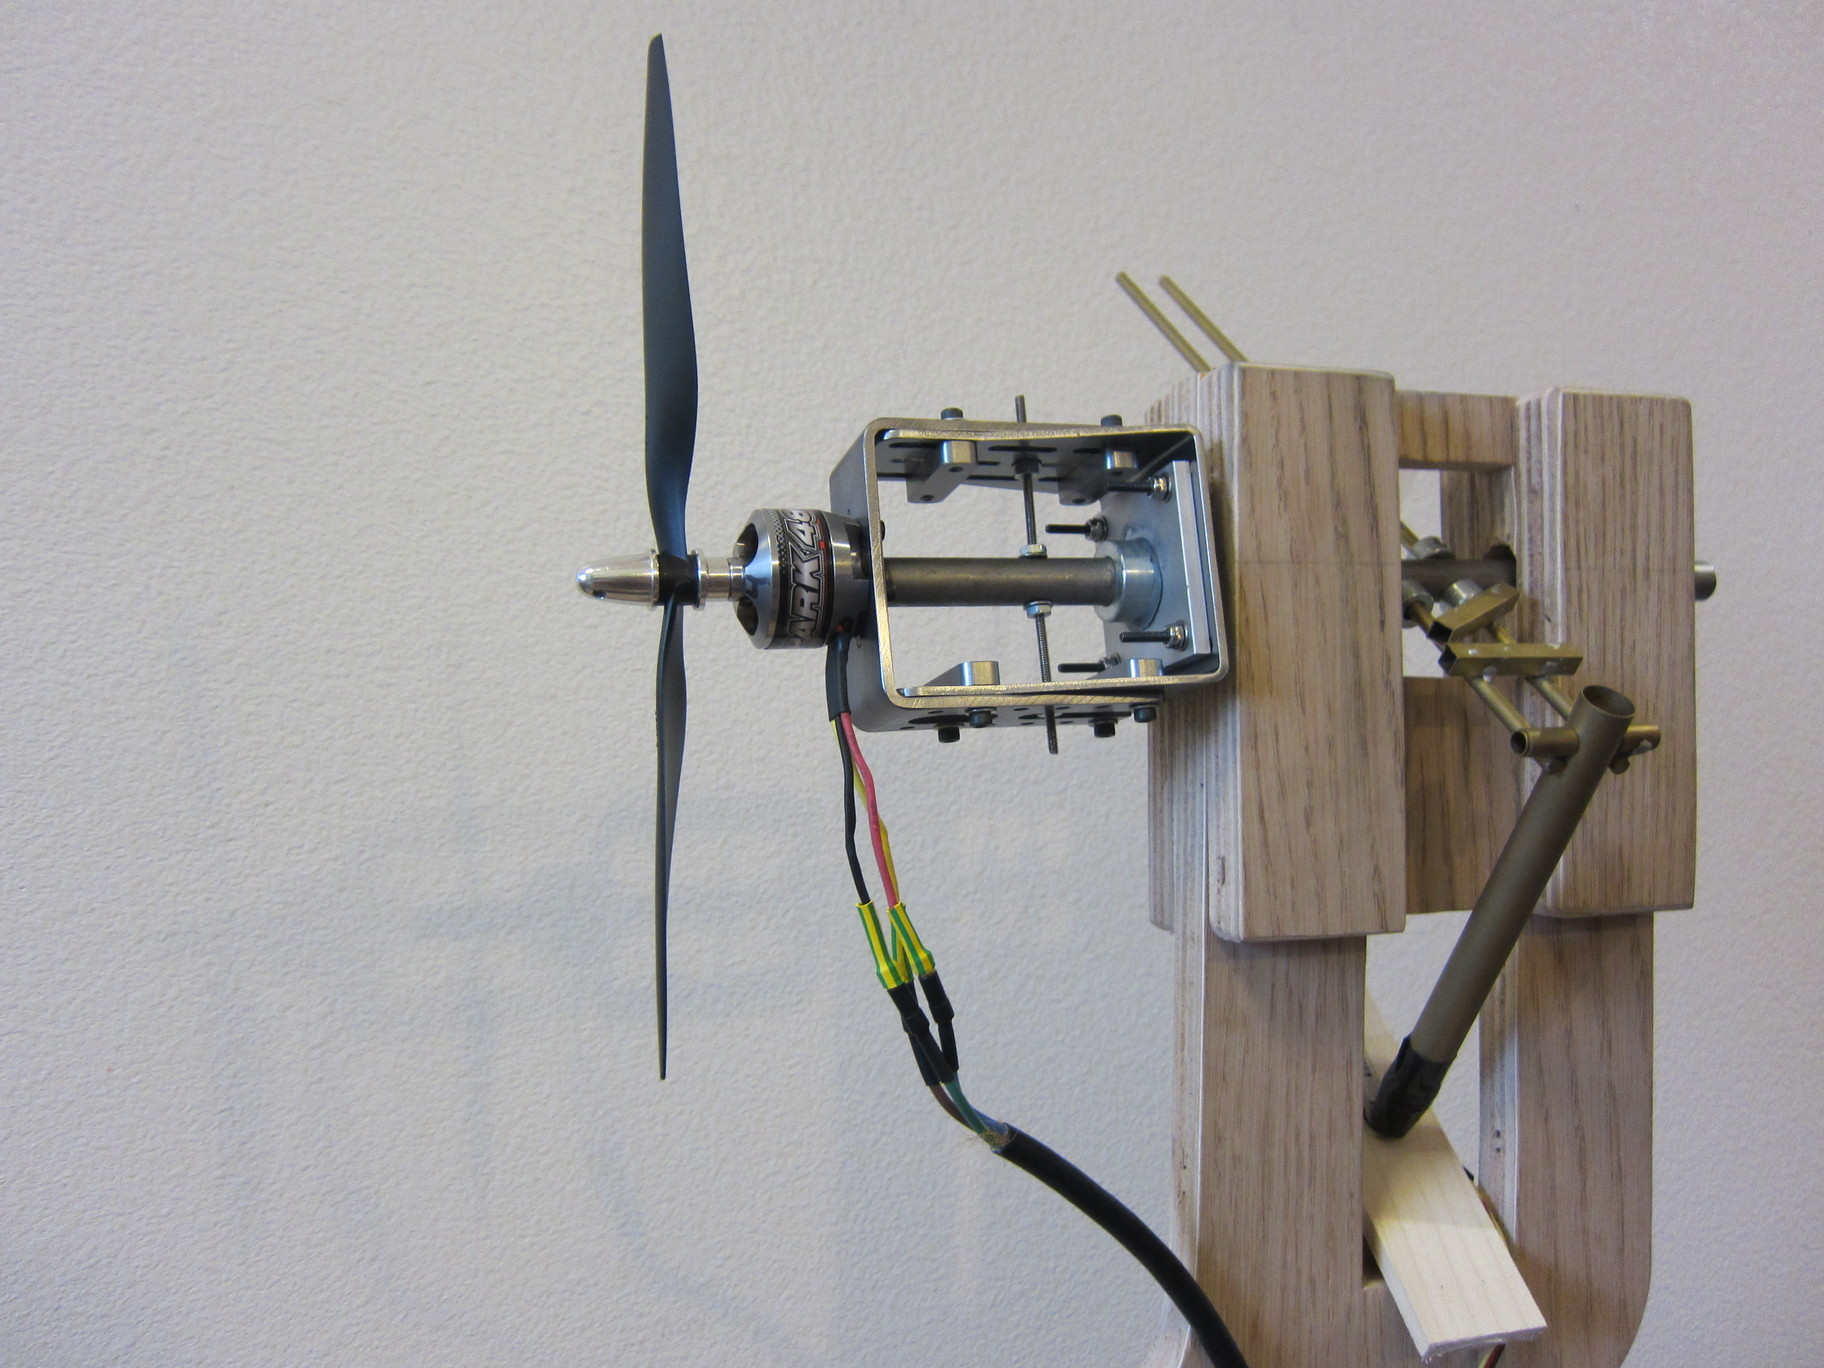
\includegraphics[scale=.22]{thrust_torque_stand_detail}
}
\caption[Optional caption for list of figures]{Brushless motor test stand}
\end{figure}

As the propeller spins, it creates a thrust force pointing to the left in the picture. This thrust force is measure by a pressure sensor on the bottom foot. Additionally, the propeller creates a torque. This torque pushes the brass lever arm into another pressure sensor on the upper part of the arm, which can then measure the motor torque.


\subsection{Software}
Most software development to this point has been to work on the various library objects, and to understand the system. In this section various significant software modules are discussed.
\subsubsection{Rotation Speed}
In order to determine the amount of thrust that a motor is producing the platform must be able to measure the RPM of the motor. For a normal two wire DC motor the only solution would be to use some sort of optical sensor to watch the motor rotate and to count the number of rotations. Usually this is done with an IR sensor that either senses a black stripe on the can of the motor, or watches the propeller and detects as it passes over a sensor. 

With a brushless motor, another option is available: monitoring the control pulses. A brushless motor has three control lines that go into the motor, and to make the motor spin the lines are pulsed in a specific order. The  timing of the pulses determine the speed of the motor, and the pulses must match the position of the motor rotor. Modern brushless motor controller chips (ESCs: Electronic Speed Controllers) have circuitry built into them that can automatically sense the position of the motor rotor and in theory could be used by a host microcontroller to determine motor rotation speed. Unfortunately, most ESCs don't provide this sort of information to a host, so it is necessary to measure the pulses directly and infer from the control pulses instead. 

A brushless motor sensor has several advantages over other methods:
\begin{list}{*}{}
	\item It is unaffected by optical conditions
	\item Mounting the sensor is considerably easier
	\item The sensor can give the true no-load rotation speed
	\item No modification to the existing motor or it's circuits is necessary
\end{list}

The Eagle Tree Brushless RPM sensor (\cite{eaglerpm}) is the only ready made solution on the market to measure the brushless motor control pulses. It is a very small device, priced at about \$12 a piece, and it can sense the rotation rate of a single motor. The sensor converts the brushless motor signals to a series of pulses where each pulse is proportional to a rotation. The Propeller does not measure the signal directly from a brushless motor control line because there are very high voltages and back EMF from the motor which creates a very nasty environment for the 3.3v microcontroller.

The Propeller object for this sensor is based on code provided by Tim Moore \cite{eaglerpmobject} . For this project, interface modifications to the object were made to the code in order to permit the reading of rotations per second. The object can support up to eight brushless motor sensors. 

\begin{figure}[ht]
\centering
\subfigure[The Eagle Tree brushless RPM sensor]{
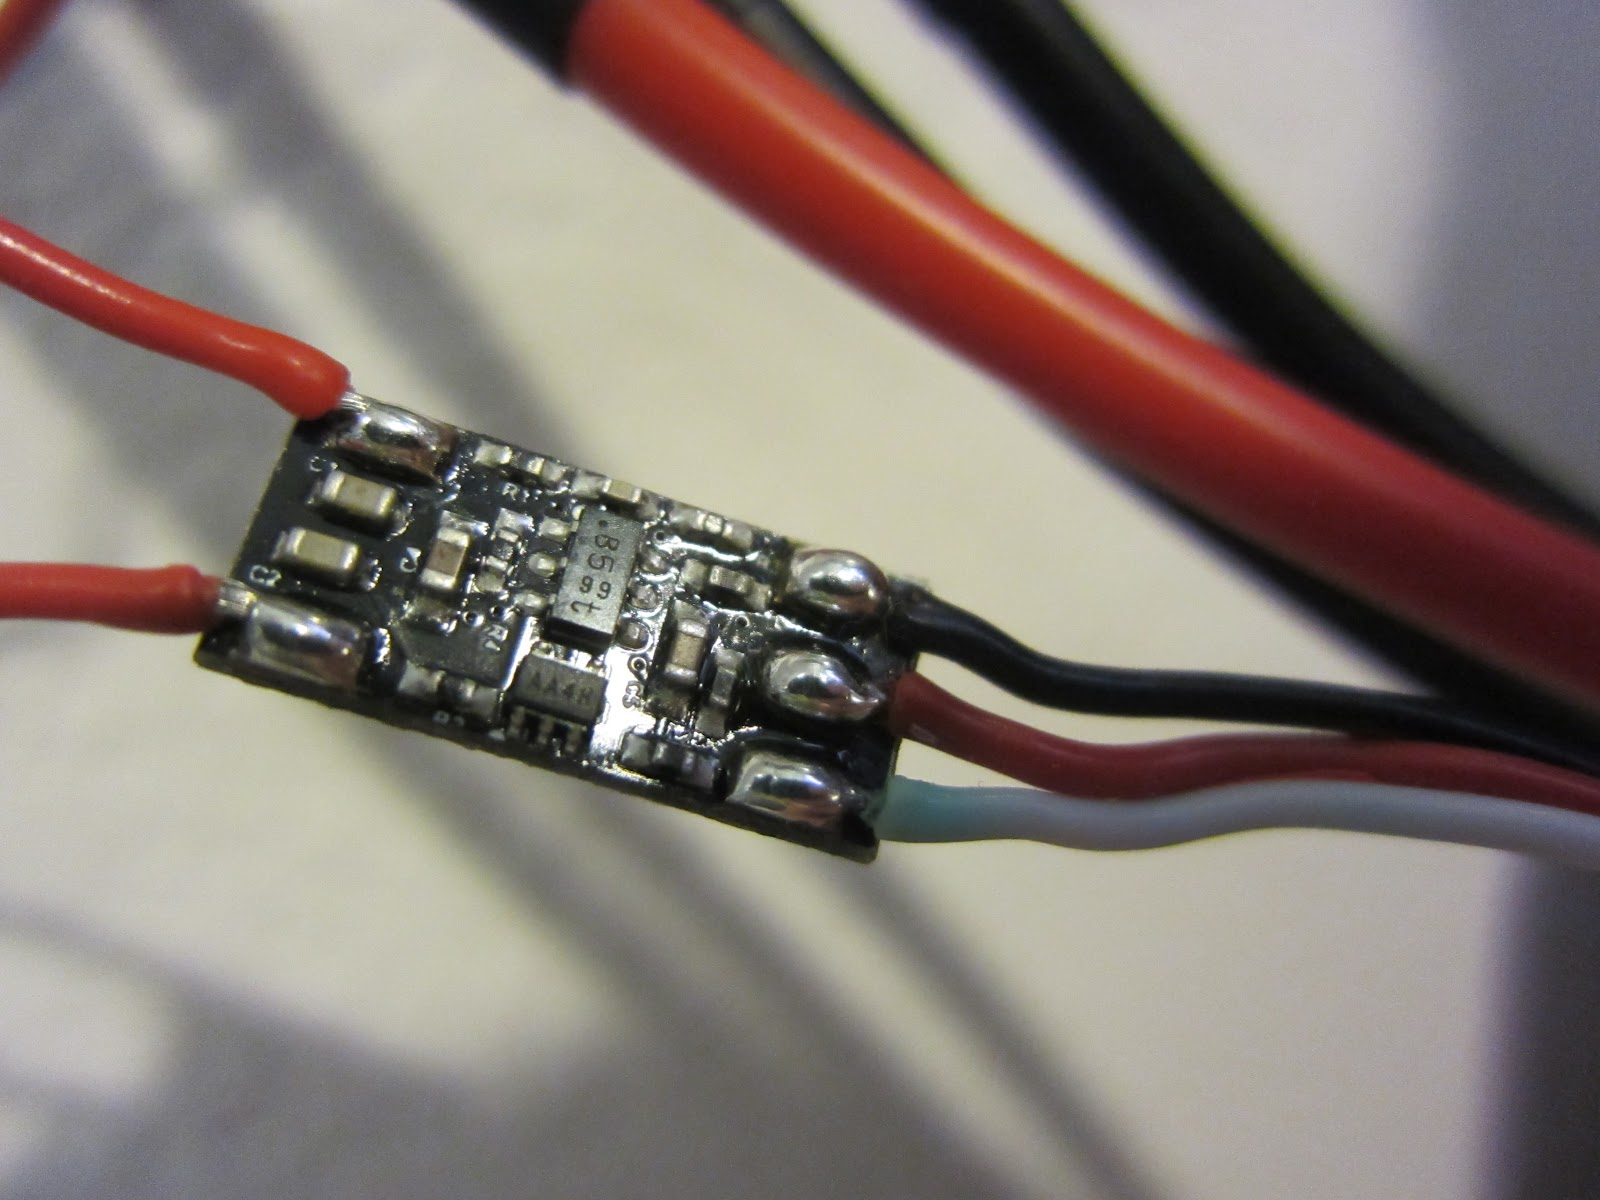
\includegraphics[scale=.1]{eagle_tree_sensor.JPG}
}
\subfigure[Motor connection of the sensor.]{
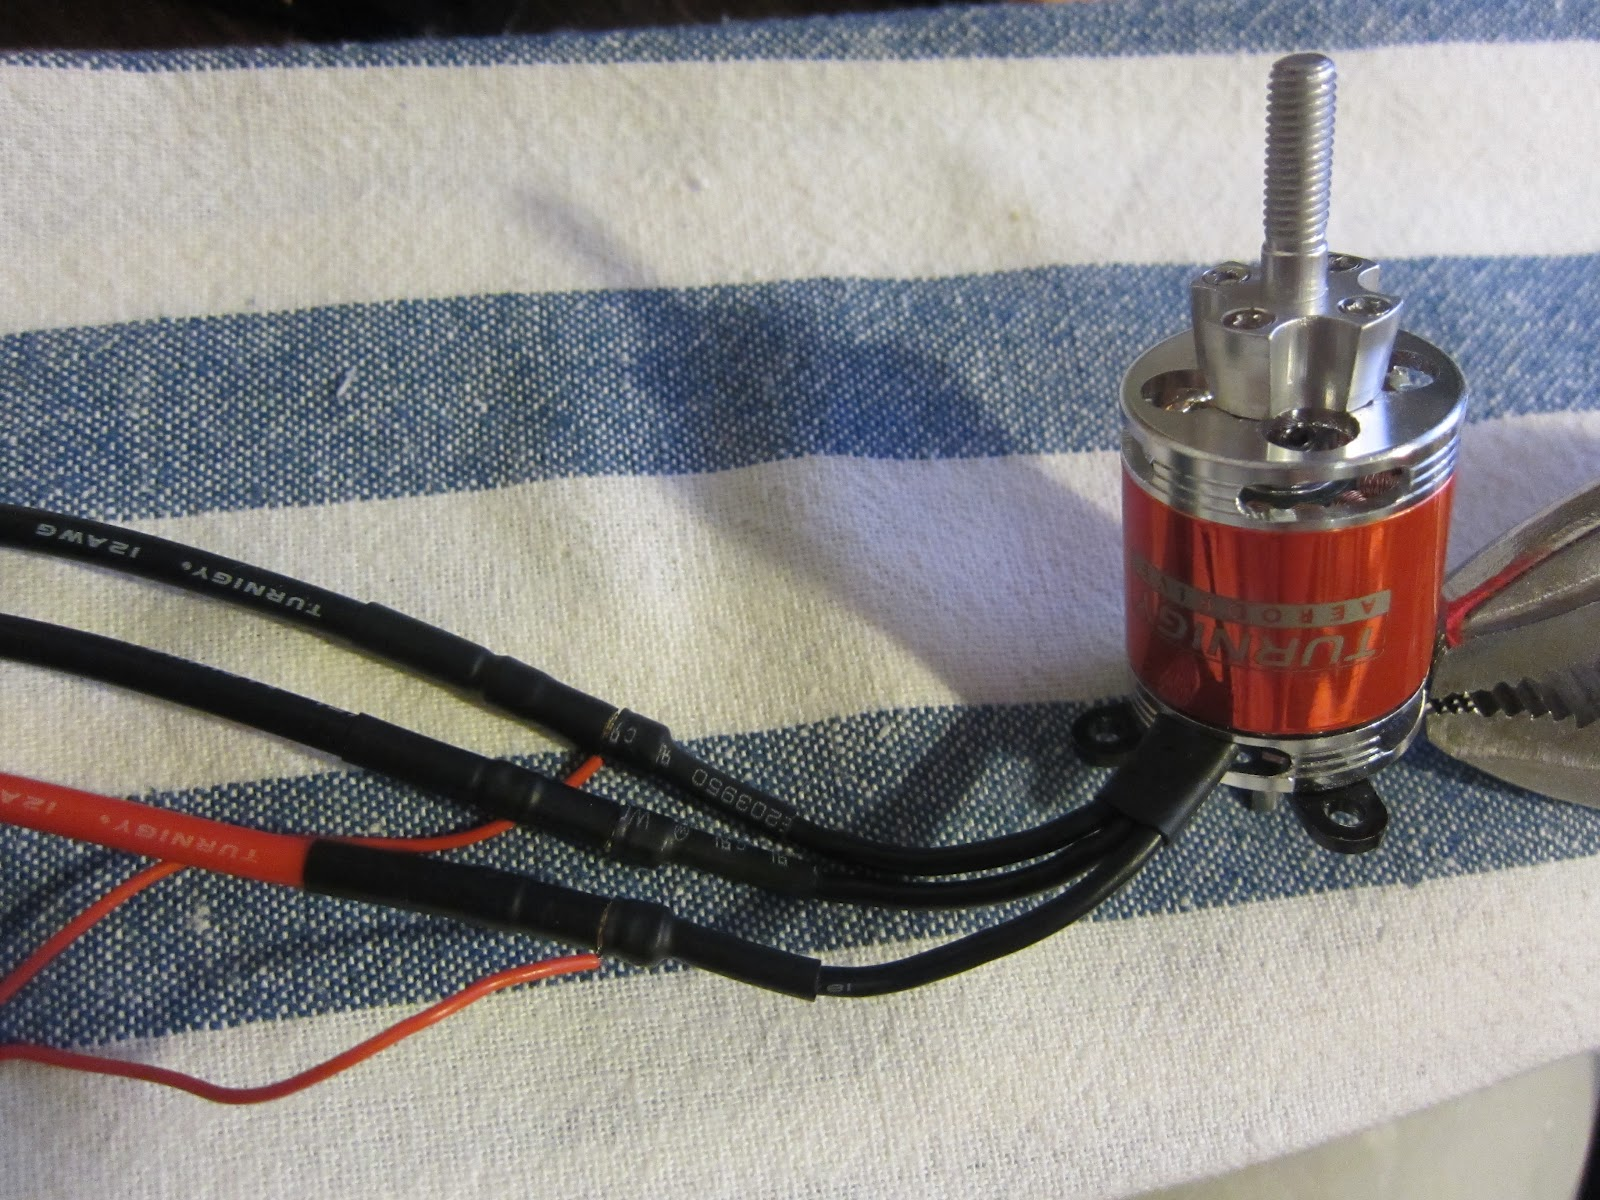
\includegraphics[scale=.1]{eagle_tree_connection.JPG}
\label{fig:subfig2}
}
\label{fig:subfigureExample}
\caption[Optional caption for list of figures]{The Eagle Tree sensor}
\end{figure}



Connection of the Eagle Tree sensor is straightforward. The two single wires from the Eagle Tree are connected to any two leads of the brushless motor. Connecting only one lead would still allow the sensor to function, but it results in slightly larger errors (15 rps errors, instead of 10 rps errors with both). On the microcontroller side the black line goes to 3.3V, red to Gnd, white to the Propeller I/O pin. Despite going against standard color coding conventions, the red line is connected to ground and the black is to 3.3v (the Propeller VDD). 

The Propeller object for interfacing with the sensor counts the number of clock cycles between rising edges of a pulse, and uses this to calculate the rotations per second.

\subsubsection{Pulse Width Modulation}
Pulse width modulation is the technique of toggling a digital I/O pin high and low in a repeating pattern. We use PWM in this project to interface the the electronic speed controllers (ESC). The ESCs use servo type PWM signals: a 1000 us to 2000 us pulse every 20 ms. The width of the pulse is relative  to the commanded speed. 


\subsubsection{UART Serial Communication}
Serial communication in this project uses the FullDuplexSerial4portPlus v3 object. This object can support up to four full duplex serial ports, although currently only one port is being used. The Propeller uses serial communication to interface to several devices:
\begin{list}{*}{}
	\item Host computer via USB
	\item Wireless modem (such as Xbee)
	\item GPS
	\item Other microcontrollers
	\item UART sensors
\end{list}
When communicating with a host computer or other microcontrollers, the Propeller uses the \$ATXXX communications protocol described in \ref{subsec:anzhelkadataandcommandexchangeprotocol}.


%% S1 S1 S1 S1 S1 S1 S1 S1 S1 S1 S1 S1 S1 S1 S1 S1 S1 S1 S1 S1  
\section{Constant Identification}
The quadrotor platform has a number of different constants that depend on the hardware used. Most constants such as mass and rotor diameter are relatively easy to measure. Other constants are not so easy. This section details the more difficult constant identifications. For a full treatment of the math and a list of all constants, see the Anzhelka mathematics document \cite{anzhelka_math}.
%% S2 S2 S2 S2 S2 S2 S2 S2 S2 S2 S2 S2 S2 S2 S2 S2 S2 S2 S2 S2  
\subsection{Thrust/Torque Test Stand Theory}

A good autonomous quadrotor needs to be able to measure, in real units such as kilograms and seconds, important aspects about itself such as orientation, motor thrust, acceleration, and so on. It's fairly easy to make a remote controlled quadrotor platform since the human in the loop can intuitively correct for many small errors, and our eyes are very good at collecting the necessary raw information. An autonomous quadrotor does not have this luxury, and must explicitly define each kinematic and dynamic equation. Among others, the quadrotor must know the propeller torque and thrust constants. 

\begin{equation} \label{eq:motor_thrust}
K_T = \frac{T}{\rho n^2 D^4}
\end{equation}

\begin{equation} \label{eq:motor_torque}
K_Q = \frac{Q}{\rho n^2 D^5}
\end{equation}

Above, we have the two equations that define how the propellers affect our quadrotor system. These equations can be found in context in the Anzhelka Project quadrotor mathematics document (\cite{anzhelka_math}). The form that \ref{eq:motor_thrust} and \ref{eq:motor_torque} are in now makes it convenient for us to measure the constants $K_T$ and $K_Q$: if we can somehow measure the terms on the right hand side then we can figure out what the constants are.

From these equations, it is clear that we need to measure thrust, torque, air density, rotation speed, and the propeller diameter. Measuring rotor diameter, motor speed and air density are straight forward, and so they are not covered here. The real challenge comes from measuring motor thrust and torque.

Thrust is measured by mounting the motor on the end of the lever arm, then measuring the torque that the propeller exerts as it spins. A pressure sensor rigidly mounted between the lever arm and a stationary base can measure this torque.

Calculating torque is a bit more complicated: the motor body needs to be mounted on a rotating axis that is directly in line with the motor shaft, and the torque along this axis needs to be measured. Most measurement test stands seem to only measure thrust, and ignore yaw. We, however, rely on the torque to yaw the quadrotor vehicle.

To measure torque, our test stand has the motor mounted to a rod, which then has a lever arm attached that presses on a scale. In a same way as thrust the force pressing on the scale can be read, and with the length of the lever arm torque can be calculated.

Our test can measure thrust and torque simultaneously and automatically. To do this we are using the Flexiforce pressure sensors (\cite{tekscanforce}). These sensors vary the resistance based on the amount of pressure, and resistance is very easy to measure with a microcontroller.

For motor speed we will be using a Eagle Tree brushless RPM sensors \cite{eaglerpm}. Our main control board is the power board that we have developed for our quadrotor. This has the advantage of being identical to what we will be flying, it will have the motor current and voltage sensing built in.
%% S2 S2 S2 S2 S2 S2 S2 S2 S2 S2 S2 S2 S2 S2 S2 S2 S2 S2 S2 S2  


%% S1 S1 S1 S1 S1 S1 S1 S1 S1 S1 S1 S1 S1 S1 S1 S1 S1 S1 S1 S1  

%% S1 S1 S1 S1 S1 S1 S1 S1 S1 S1 S1 S1 S1 S1 S1 S1 S1 S1 S1 S1  
\section{Implementation Details}
This section describes various details necessary for the project successfully run.

\subsection{Anzhelka Data and Command Exchange Protocol} \label{subsec:anzhelkadataandcommandexchangeprotocol}

%\subsubsection{Introduction}
The Anzhelka project uses a protocol called \$ATXXX to facilitate data and command exchange between different subsystems. \$ATXXX is very similar to NMEA-0183 where data is exchanged via sentences prefaced with a sentence code. This allows for the Propeller to send real time information about the running state to other onboard processors or to offboard computers, and to receive commands. The protocol was developed to facilitate predictable and reliable exchanges.

\subsubsection{Protocol Implementation Details}
All strings are encoded in standard ASCII. Numbers are converted to their ASCII equivalent and are in base 10 unless otherwise noted. If a number is a decimal then it will have the ASCII decimal point included in the sentence string. By having all the data be in ASCII a normal terminal program (such as picocom or cutecom) can be used to receive and send data. 

Each string is independent of all other strings. There is no order required to send or receive strings. If multiple strings of the same type are received, the listening devices should assume that the last received is the most recent. If an unknown string or other serial data is encountered then it should be ignored.

Data strings are prefaced with \$ADxxx (short for Anzhelka Data type xxx). 

Note that the only defined whitespace in a string is a single space after the sentence code, and a newline (ASCII characters LF and CR) after each string. For clarity of notation the newline is not written in the string lists below.

\subsubsection{Example Usages}
This protocol is used in the thrust/torque test stand. The test stand measures the thrust and torque using force sensors, and measures the rotations per second of the motor. The test stand then outputs the \$ADRPS, \$ADPWM, \$ADMTH, and \$ADMTQ strings to a USB serial port. A desktop computer reads these strings from the serial port and displays the variable on-screen in a GUI that updates in real time as new strings are received. In this way the user can watch as testing proceeds.

This protocol could also be used to log parameters of the quadrotor as it is flying. The Propeller that is controlling the quadrotor could send these strings via a serial port to an external SD card. If an SD card is not available then the system could perhaps use a wireless transceiver such as an XBee. In the event of a system failure, the developer could look at the logged strings in order to help with debugging. 


\subsubsection{Protocol String Table}
\begin{longtable}{p{2cm}p{9cm}}
\hline
\$ADRPS &
	Most recent rotations per second for each motor \newline
	Format: \newline
	\texttt{\$ADRPS m1,m2,m3,m4} \\ 
\hline
\$ADMIA &
	Most recent motor current in milliamps \newline
	Format: \newline
	\texttt{\$ADMIA m1,m2,m3,m4} \\
\hline
\$ADMVV &
	Most recent motor voltage in millivolts \newline
	Format: \newline
	\texttt{\$ADMVV m1,m2,m3,m4} \\
\hline
\$ADPWM &
	Most recent motor PWM command, in microseconds (uS) \newline 
	Format:  \newline
	\texttt{\$ADPWM m1,m2,m3,m4} \\
\hline
\$ADMKP &
	Current motor PID loop proportional constant (KP). No units.  \newline
	Format:  \newline
	\texttt{\$ADMKP m1,m2,m3,m4} \\
\hline
\$ADMKI &
	Current motor PID loop integral constant (KI). No units.  \newline
	Format:  \newline
	\texttt{\$ADMKI m1,m2,m3,m4} \\
\hline
\$ADMKD &
	Current motor PID loop derivative constant (KD). No units.  \newline
	Format:  \newline
	\texttt{\$ADMKD m1,m2,m3,m4} \\
\hline
\$ADMTH &
	Most recent motor thrust in units of Newtons.  \newline
	Format:  \newline
	\texttt{\$ADMTH m1,m2,m3,m4} \\
\hline
\$ADMTQ &
	Most recent motor torque in units of Newton-Meters.  \newline
	Format:  \newline
	\texttt{\$ADMTQ m1,m2,m3,m4} \\
\hline
\$ADDRP &
	Most recent motor rotations per second set point (the desired rps). This is the speed that motors are trying to achieve, and is fed into the motor PID loops. 
	Format: 
	\texttt{\$ADDRP m1,m2,m3,m4} \\
\hline
\end{longtable}


%% S1 S1 S1 S1 S1 S1 S1 S1 S1 S1 S1 S1 S1 S1 S1 S1 S1 S1 S1 S1  

%% S2 S2 S2 S2 S2 S2 S2 S2 S2 S2 S2 S2 S2 S2 S2 S2 S2 S2 S2 S2  
%\subsection{High Level Hardware Design}
%\textcolor{red}{Luke}
%TO DO: Highlevel hardware design


%% S2 S2 S2 S2 S2 S2 S2 S2 S2 S2 S2 S2 S2 S2 S2 S2 S2 S2 S2 S2  

%% S2 S2 S2 S2 S2 S2 S2 S2 S2 S2 S2 S2 S2 S2 S2 S2 S2 S2 S2 S2  
%\subsection{High Level Software Design}
%\textcolor{red}{Cody}
%TO DO: Highlevel software design
%% S2 S2 S2 S2 S2 S2 S2 S2 S2 S2 S2 S2 S2 S2 S2 S2 S2 S2 S2 S2  

 
%% S1 S1 S1 S1 S1 S1 S1 S1 S1 S1 S1 S1 S1 S1 S1 S1 S1 S1 S1 S1  
\section{User Interface Design}
Currently, the only user interface is via the Anzhelka Terminal.
%% S1 S1 S1 S1 S1 S1 S1 S1 S1 S1 S1 S1 S1 S1 S1 S1 S1 S1 S1 S1  

%% S2 S2 S2 S2 S2 S2 S2 S2 S2 S2 S2 S2 S2 S2 S2 S2 S2 S2 S2 S2  
\subsection{Anzhelka Terminal}
\begin{figure}[h!]
\centering
	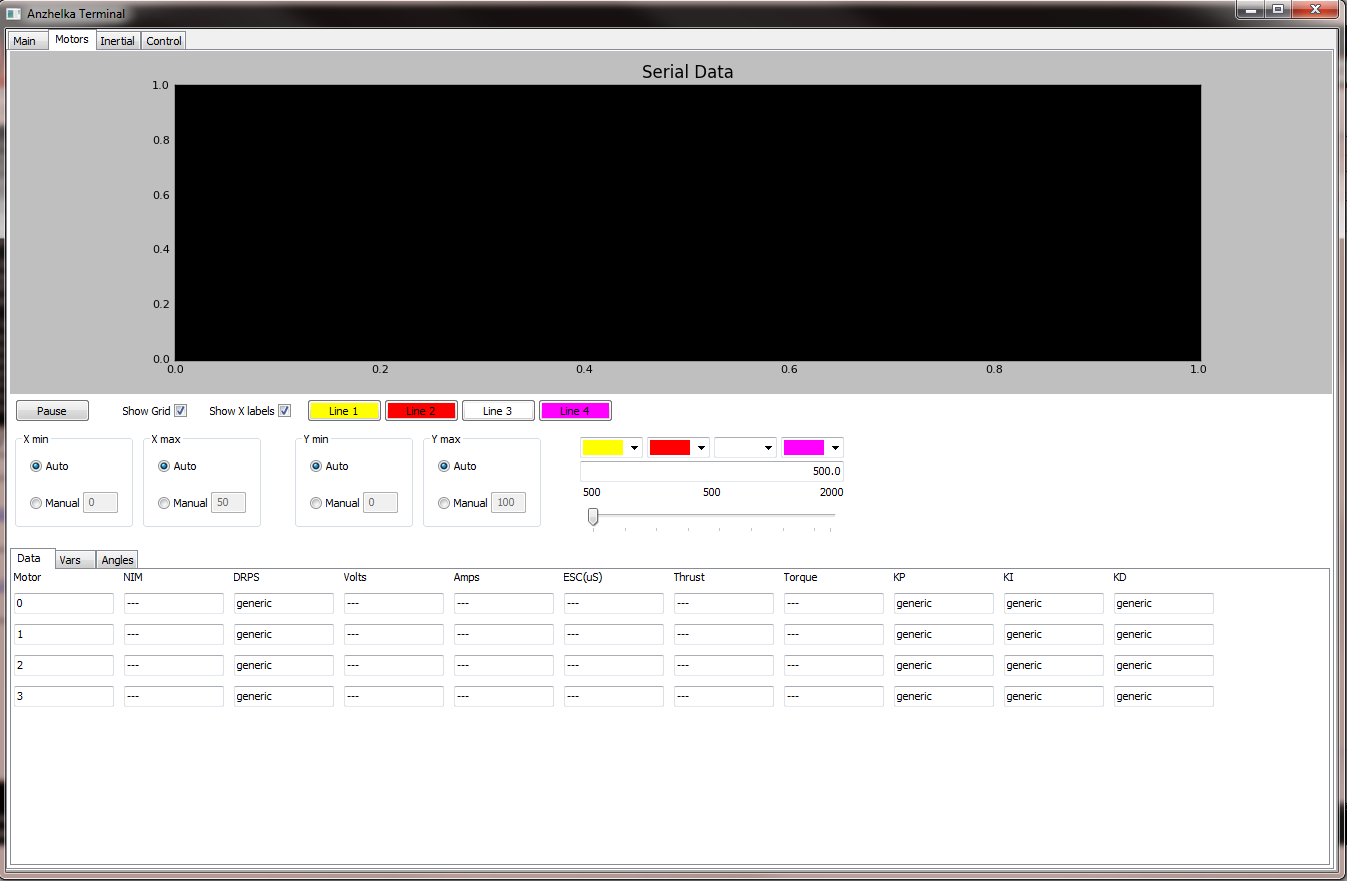
\includegraphics[scale=.33]{anzhelka_terminal_data.png}
\end{figure}

The Anzhelka project uses a PC based GUI platform called Anzhelka Terminal (AT) to display realtime system states and to allow for parameter tuning. AT is written in Python and uses the WxWidgets Python branch WxPython for the GUI. AT is cross platform.

The AT GUI was written in WxPython and developed in part with the WYSIWYG editor WxGlade. WxGlade was suitable for most of the general layout tools, but was insufficient in two areas. First, WxGlade could not specifically layout the dynamic graphs since the graph class is a non standard class. Secondly, WxGlade was not used to layout the motor parameter table. This table has a row for each motor (normally 4 motors, but possibly 3 or more) and a column for each parameter of interest. Since this section was hand coded, either number should be easily changeable without excessive GUI editing .

AT will listen on the specified serial port for \$ATXXX strings, and will  make these strings available for reading. Within the program, different threads will search the received strings list and extract the strings of interest, then display them onscreen. If an unknown string is encountered then AT will ignore it.

There are two GUI screens that are currently implemented: the COM port setup tab and the motor variable tab. Additional screens planned for the future include a inertial measurements tab, a control parameters tuning tab, and a high level command tab.

The motor control tab has several features that are important. At the top of the pane is a dynamic graph that will display in real time it's received information. This feature was one of the deciding factors to use Python instead of some other language. The graph can be automatically or user scaled on either axis, and is updated behind the scenes with the received serial strings.

Below the graph is the motor parameter table. This table displays all relevant information about each motor, including: 
motor number
rotations per second
desired rotations per second
voltage
current
electronic speed controller PWM command
thrust
torque
$K_P$ of the motor PID controller
$K_I$ of the motor PID controller
$K_D$ of the motor PID controller
The table is updated in real time based on the received strings. Some fields are editable as well (such as $K_{PID}$ and DRPM), and when changed AT will send these values through the serial port as a \$ATXXX string (Note: this feature is still in development). This table is generated at runtime so it is easy to change the number of motors and the motor parameters. This was done in particular to support the same AT program for hexrotors and octorotors as well as quadrotors.
%% S2 S2 S2 S2 S2 S2 S2 S2 S2 S2 S2 S2 S2 S2 S2 S2 S2 S2 S2 S2  



%% S1 S1 S1 S1 S1 S1 S1 S1 S1 S1 S1 S1 S1 S1 S1 S1 S1 S1 S1 S1  

%% S1 S1 S1 S1 S1 S1 S1 S1 S1 S1 S1 S1 S1 S1 S1 S1 S1 S1 S1 S1  
\section{Testing}
Testing is a critical part of any project, and the Anzhelka project is no exception. All hardware and software is tested thoroughly to ensure correctness. As more time passes we will work on developing automated tests, including regression tests once the project becomes mature.
%% S1 S1 S1 S1 S1 S1 S1 S1 S1 S1 S1 S1 S1 S1 S1 S1 S1 S1 S1 S1  

%% S2 S2 S2 S2 S2 S2 S2 S2 S2 S2 S2 S2 S2 S2 S2 S2 S2 S2 S2 S2 
%\subsection{Software Testing}
%% S2 S2 S2 S2 S2 S2 S2 S2 S2 S2 S2 S2 S2 S2 S2 S2 S2 S2 S2 S2 

%% S3 S3 S3 S3 S3 S3 S3 S3 S3 S3 S3 S3 S3 S3 S3 S3 S3 S3 S3 S3
%\subsubsection{Unit Testing}
%\textcolor{red}{Cody}
%% S3 S3 S3 S3 S3 S3 S3 S3 S3 S3 S3 S3 S3 S3 S3 S3 S3 S3 S3 S3

%% S3 S3 S3 S3 S3 S3 S3 S3 S3 S3 S3 S3 S3 S3 S3 S3 S3 S3 S3 S3
%\subsubsection{Integration Testing}
%\textcolor{red}{Cody}
%% S3 S3 S3 S3 S3 S3 S3 S3 S3 S3 S3 S3 S3 S3 S3 S3 S3 S3 S3 S3

%% S3 S3 S3 S3 S3 S3 S3 S3 S3 S3 S3 S3 S3 S3 S3 S3 S3 S3 S3 S3
%\subsubsection{Acceptance Testing}
%\textcolor{red}{Cody}
%% S3 S3 S3 S3 S3 S3 S3 S3 S3 S3 S3 S3 S3 S3 S3 S3 S3 S3 S3 S3

%% S2 S2 S2 S2 S2 S2 S2 S2 S2 S2 S2 S2 S2 S2 S2 S2 S2 S2 S2 S2 
\subsection{Hardware Testing}
Because hardware is a physical entity it is subjected to many more points of failure. Parts can be flawed from the factory, assembled wrongly, or miscalculated.
%% S2 S2 S2 S2 S2 S2 S2 S2 S2 S2 S2 S2 S2 S2 S2 S2 S2 S2 S2 S2 

%% S3 S3 S3 S3 S3 S3 S3 S3 S3 S3 S3 S3 S3 S3 S3 S3 S3 S3 S3 S3
\subsubsection{Frame}
The frame is rigid and is made up from nearly the same exact components for all 4 booms. The center of the frame is the only thing that is not duplicated, however the top side and bottom side are nearly identical with minor mounting differences and the center plates are symmetric about the $z$ axis. Each boom needs to be identical in both size and weight to ensure proper balancing.

Once each boom is assembled it should weigh identically to the other booms. If there is too much of a difference in the weight of the booms it could could cause the center of mass to change too dramatically. Therefore the booms must be matched.
%% S3 S3 S3 S3 S3 S3 S3 S3 S3 S3 S3 S3 S3 S3 S3 S3 S3 S3 S3 S3

%% S3 S3 S3 S3 S3 S3 S3 S3 S3 S3 S3 S3 S3 S3 S3 S3 S3 S3 S3 S3
\subsubsection{Motors/Propellers}
The motors and propellers would also need to be tested and matched to ensure the best performance. We can assemble all of our motors and propellers and then we can test them for torque and thrust ratings. Once we have all of the results we can then match the motors with nearly the same characteristics together.

One slight nick in a propeller can cause a large vibration problem that can affect the entire quadrotor frame. If this is the case the propeller must be balanced using a magnetic propeller balancer. If it can't be balanced then the propeller must be discarded.

We know that most motors made by the same manufacture with the same specifications should be nearly identical. From this we can assume that all motors are same and can be treated as such. Additionally, by measuring the RPM most motor specific effects can be reduced or eliminated.
%% S3 S3 S3 S3 S3 S3 S3 S3 S3 S3 S3 S3 S3 S3 S3 S3 S3 S3 S3 S3

%% S3 S3 S3 S3 S3 S3 S3 S3 S3 S3 S3 S3 S3 S3 S3 S3 S3 S3 S3 S3
\subsubsection{PCBs}
PCBs can have many points of failure and need to be tested at many different parts of the build phase to ensure the most amount of yield. 

Each fabrications house has its own set of limitations on what it can produce as far as trace widths, via sizes, spacing, etc. All fabrication houses will provide you with these details before you place an order so that you know what you can and what you can't do in your design. You must also keep in mind the amount of current  or power that will have to travel through your traces that you have designed onto your board. If you are trying to push 10 amps through a 6mil trace you are going to melt the trace and ruin your board. Designers must take care to check and double check these considerations. 

Once you have sent off your design to the fabrication house to be produced, the product must then be electrically tested. Electrical testing is a key factor in product yield. What is electrical testing? Electrical testing is a process in testing that checks whether a pad that is supposed to be electrically connected to another pad is actually connected. This may sound quite simple; however, in practice boards can have thousands of points that need to be tested. Some fabrication houses will provided 50\% to 100\% electrical testing, others will not provide any testing at all. 

In the event that you can not get your boards fully tested you will need to create an overlay that will touch all the pads and check to see what is connected and what is not. In practice this is not acceptable to be done outside of the fabrication house or other than a special electrical testing board house.

The physical components that will be soldered onto the PCB have usually been tested and have an acceptable failure rate that will not have a great effect on the yield. With that being said, placement of the components is essential. If a component is misplaced by 20mils this could cause a bridge between two pins causing a short rendering that board unusable.

Once the PCB has been fully populated it now must be tested to ensure that all the components are in working order. One of the easiest ways to accomplish this is to develop test code that will run on the hardware and will give you a set of known outputs. Having something that will test all components several times under different inputs and outputs is key to ensure that the PCB is in good working order.
%% S3 S3 S3 S3 S3 S3 S3 S3 S3 S3 S3 S3 S3 S3 S3 S3 S3 S3 S3 S3

%% S1 S1 S1 S1 S1 S1 S1 S1 S1 S1 S1 S1 S1 S1 S1 S1 S1 S1 S1 S1  
\section{Maintenance Plan}
We will continue to work on and develop this project for the rest of the school year, and with any luck beyond the end of the year. The current status of the project can always be found at the project blog (\cite{anzhelka_blog}).
%% S1 S1 S1 S1 S1 S1 S1 S1 S1 S1 S1 S1 S1 S1 S1 S1 S1 S1 S1 S1  

%% S2 S2 S2 S2 S2 S2 S2 S2 S2 S2 S2 S2 S2 S2 S2 S2 S2 S2 S2 S2  
\subsection{For the next ten weeks} \label{subsec:maintenance_plan_10}
This senior design project is no where it needs to be as for a finished product and will require a lot more time to get there. In the following weeks we hope to accomplish the following tasks:

\begin{list}{*}{}
	\item Write motor PID object
	\item Calibrate the pressure sensors for the test stand
	\item Characterizing the Motors and Propellers
	\item Create Eagle Tree wiring harnesses
	\item Finalize mechanical assembly
	\item Mount the IMU onto the quadrotor
	\item Write the IMU interface object
	\item Set up wireless interfacing
	\item Balancing of the propellers
	\item Build Roll and Pitch test stand
	\item Write Motor control object
	\item Finish all electrical wiring for the quadrotor
	\item Write attitude control object
	\item Build yaw test stand
	\item Write altitude control object
	\item Test for physical limit of payload capacity
\end{list}
These are just some of the many items that we hope to complete in the following ten weeks.

%% S2 S2 S2 S2 S2 S2 S2 S2 S2 S2 S2 S2 S2 S2 S2 S2 S2 S2 S2 S2  

%% S2 S2 S2 S2 S2 S2 S2 S2 S2 S2 S2 S2 S2 S2 S2 S2 S2 S2 S2 S2  
\subsection{For the next year}
Since the members of this project are so financially invested into it, we plan on continuing this project for a very long time. It is quite possible that we may even turn this project into company or a business.

One of the hopes is to present the project to the investor community(Kickstarter, IndieGoGo, etc.) and to see if there is enough interest in the project to have them help fund this idea to its full potential.

With the right funding we could add things like object avoidance, quadrotor acrobatics, and other ideas provided by users.
%% S2 S2 S2 S2 S2 S2 S2 S2 S2 S2 S2 S2 S2 S2 S2 S2 S2 S2 S2 S2  

%% S1 S1 S1 S1 S1 S1 S1 S1 S1 S1 S1 S1 S1 S1 S1 S1 S1 S1 S1 S1  
\section{Engineering Effort and Societal Impacts}
Every project has an effect on other people, and autonomous quadrotors are no different.

\subsection{Realistic Constraints on Time and Money}

The Anzhelka project is relatively unconstrained in time and money. We each work roughly 20-40 hours a week on the project, for a total of 23 weeks. This gives approximately 1400 hours of total time investment in the project. Many other students are unwilling or unable to invest as much time as we have in our project. Once the project is accepted by the open source community it should become self sustaining by volunteers. Most likely these volunteers will come from the Parallax forums, since that is the main source of Propeller based collaboration.

This project is also relatively unconstrained in terms of finances. We have invested roughly \$3000 in this project to get it started and off the ground. This money is from savings. Like the amount of time we invest in the project, many other students are unwilling or unable to invest as much money as we have done. We were able to invest as much as we have by preparing and saving for the project before it actually began. It is no surprise that a senior design project was required before graduation.

\subsection{Safety and Reliability}

Safety and Reliability are very important for this project. This project conforms to the Remote Control Aerial Photography Association general operation guidelines (\cite{rcapa_guidelines}). These guidelines give rules for safe operation of remote controlled vehicles. 

\subsection{Aesthetics}
\begin{figure}[h!]
  \centering
	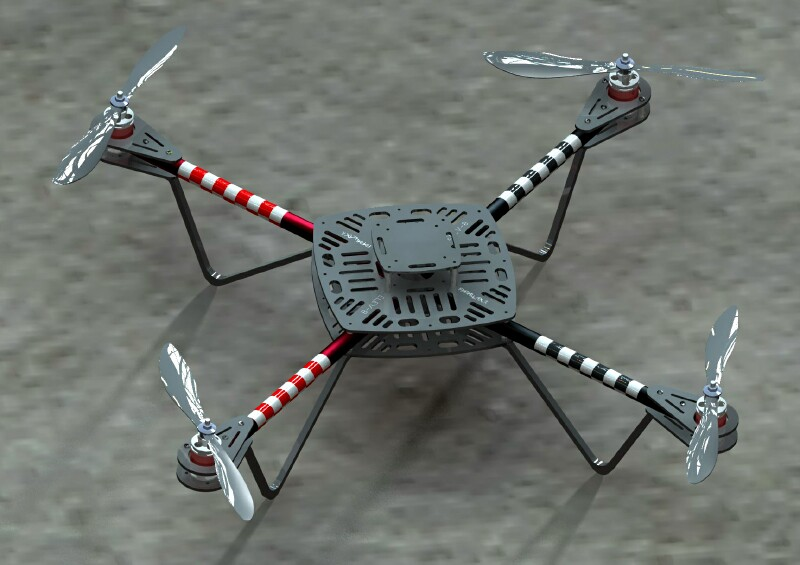
\includegraphics[scale=.35]{elev_8_artistic_rendering.jpg}
  \caption{An artistic rendering of the Elev-8 frame.}
\end{figure}  

The Elev-8 platform is very aesthetic. It has appeal simply for it's uncommon design that many people are unfamiliar with. Quadrotors in general are very popular for their novelty. The commercial Parrot AR Drone quadrotor has a booth every year at the Consumer Electronics Show in Las Vegas, and every year it is packed with spectators.

Several steps were taken to improve the general aesthetics of the quadrotor frame. All wiring was kept to a minimum and hidden wherever possible. The PCB was designed to reduce the number of external components that had to be connected with messy wires. All screws are black oxide coated to match the black of the Delrin pieces. The PCB has a white solder mask to contrast with the black color of the frame.

The Anzhelka Terminal GUI was designed to be intuitive and easy to use, even without any experience. Functionality is divided into tabs for easy access. The motors tab allows for intuitive control of the graph, and the motor table is clear and easy to understand. 

The thrust/torque test stand also had aesthetics in mind when it was designed. The stand is build out of oak and finished in a way that makes the wood almost glow. The metal pieces were sandblasted to create a matte finish. Finally, all wiring was routed and organized as best as possible.

\subsection{Anzhelka Marketing}
We have worked on marketing this project as well. We selected the name "Anzhelka" (meaning angelic in Russian) and made it the core identifier of our project. We have developed the phoenix logo that is used on everything that we produce. We have developed team T-shirts and a display board to simultaneously educate and promote the project. We have a project domain (anzhelka.com) and sensible web addresses. This project now has an identity such as few senior design projects ever achieve.


%% S1 S1 S1 S1 S1 S1 S1 S1 S1 S1 S1 S1 S1 S1 S1 S1 S1 S1 S1 S1  

%% S1 S1 S1 S1 S1 S1 S1 S1 S1 S1 S1 S1 S1 S1 S1 S1 S1 S1 S1 S1  
\section{Conclusion and Future Work}
%% S1 S1 S1 S1 S1 S1 S1 S1 S1 S1 S1 S1 S1 S1 S1 S1 S1 S1 S1 S1

%% S2 S2 S2 S2 S2 S2 S2 S2 S2 S2 S2 S2 S2 S2 S2 S2 S2 S2 S2 S2  
\subsection{Conclusion}
For this project, we have developed the hardware and software frameworks necessary to fly autonomously. We have built and tested the mechanical and electrical hardware, and developed much of the associated sensor software. We have analysed current research papers on the topic of quadrotor control, and have developed a document that clearly and precisely outlines the steps necessary to fly (\cite{anzhelka_math}). We have extensively documented the entire process, and provided all of it as open source. We have created an identity for the project in the form of the name Anzhelka and our phoenix logo. With these accomplishments we are only a few small steps away from flying.

We were, and are constantly surprised by the amount of work even apparently simple tasks take. We had originally anticipated being able to fly by mid January. Then mid February. Now, it is mid May. The process has been a learning experience for both of us. We have learned the value of a methodical approach and good documentation, and to respect the progress of others in our field.

If we had to do it differently we would make a larger team. Specifically, it would be very beneficial to add several new roles in addition to the computer engineering and computer science roles that we already fill. A mechanical engineer would take care of the quadrotor frame, an electrical engineer would take care of the circuits, and an administration major would maintain all the documentation. With these three other people we could make the excellent project it already is absolutely outstanding.
%% S2 S2 S2 S2 S2 S2 S2 S2 S2 S2 S2 S2 S2 S2 S2 S2 S2 S2 S2 S2  


%% S1 S1 S1 S1 S1 S1 S1 S1 S1 S1 S1 S1 S1 S1 S1 S1 S1 S1 S1 S1 
\subsection{Acknowledgements}
We have had a considerable amount of assistance with this project. We would like to thank everyone who has supported us as we work on the largest undertaking either of us has ever done.
\begin{longtable}{l l}
W9GFO (Rich Harman)& Laser cutting of the Derlin\textregistered  \- Frame Parts \\
Gene Shermen & Machinist \\
Dale Holtkamp & Machinist \\
Elmar Palma & Workshop \\
Dr. Philip Brisk & Consulting \\
Dr. Ping Liang & Consulting \\
Dr. Roman Chomko & Consulting \\
Dr. Kastner & Consulting \\
Tom Wypych & Consulting \\
Frank Lewis & Algorithms \\
Emanuel Stingu & Algorithms \\
Texas Instraments & Samples \\
Microchip & Samples \\
Jack Mcbroom & Other \\
\end{longtable}
%% S1 S1 S1 S1 S1 S1 S1 S1 S1 S1 S1 S1 S1 S1 S1 S1 S1 S1 S1 S1 

%% S1 S1 S1 S1 S1 S1 S1 S1 S1 S1 S1 S1 S1 S1 S1 S1 S1 S1 S1 S1  
\section{References}

\begin{thebibliography}{99}

%Use postfix of 69 to indicate unknown year

	\bibitem{anzhelka_code}
	C. Lewis, L De Ruyter,
	\url{"http://code.anzhelka.com"}
	
	\bibitem{anzhelka_blog}
	C. Lewis, L De Ruyter,
	\url{"http://blog.anzhelka.com"}

	\bibitem{anzhelka_math}
	C. Lewis, L De Ruyter,
	"Quadrotor Mathematics For Simpletons," 2012, available at \url{"http://code.anzhelka.com"}
	
	\bibitem{stingu09}
	E. Stingu, F. Lewis, 
	"Design and Implementation of a Structured Flight Controller for a 6DoF Quadrotor Using Quaternions," 
	Mediterranean Conference on Control \& Automation, pp. 1233-1238, June 2009.
	
	\bibitem{campbell09} % http://www.fnarfbargle.com/bst.html
	B. Campbell, 
	"BST - The multi-platform Propeller Tool Suite" 
	\url{"http://www.fnarfbargle.com/bst.html"} 2009.

	\bibitem{elev8_frame}
	K. Gracey,
	Elev-8 Quadcopter, \url{"http://www.parallax.com/tabid/768/ProductID/799/Default.aspx"}
	
	\bibitem{tekscanforce} % http://www.tekscan.com/pdf/A201-force-sensor.pdf
	Tekscan\textregistered 
	\url{"http://www.tekscan.com/pdf/A201-force-sensor.pdf"}
	
	\bibitem{eaglerpm} % http://www.eagletreesystems.com/support/manuals/brushless-rpm.pdf
	Eagle Tree Systems \textregistered
	\url{"http://www.eagletreesystems.com/support/manuals/brushless-rpm.pdf"}

	\bibitem{dupontdelin} % http://www2.dupont.com/Plastics/en_US/Products/Delrin/Delrin.html
	Dupont\texttrademark
	\url{"http://www2.dupont.com/Plastics/en_US/Products/Delrin/Delrin.html"}
	
	\bibitem{eaglerpmobject} %(http://forums.parallax.com/showthread.php?127372-PWM_32_V2-Question-about-Resolution-constant)
	Tim Moore
	\url{"http://forums.parallax.com/showthread.php?127372-PWM_32_V2-Question-about-Resolution-constant"}
	
	
	\bibitem{vibration_loose}
	"Vibration Loosening of Bolts and Threaded Fasteners", 2012,
	\url{"http://www.boltscience.com/pages/vibloose.htm"}
	
	\bibitem{propeller_pitch} %Link to paper that explains maximum efficiency at small pitch.
	EPI Inc. "Propeller Performance Factors", 2010, \url{"http://www.epi-eng.com/propeller_technology/selecting_a_propeller.htm"}
	\bibitem{rcapa_guidelines}
	Remote Control Aerial Photography Association, "General Guidelines", 2012 \url{"http://www.rcapa.net/guidelines.aspx"}
	
	
	\bibitem{human_reaction_time}
	HumanBenchmark.com, 2012, \url{"http://www.humanbenchmark.com/tests/reactiontime/stats.php"}
	
	\bibitem{float32}
	C. Thompson, "Floating Point", 2009, \url{"http://obex.parallax.com/objects/202/"}
	
	\bibitem{aeroquad}
	AeroQuad, 2012, \url{http://aeroquad.com/}
	
	\bibitem{arducopter}
	DIY Drones Arducopter, 2012, \url{http://code.google.com/p/arducopter/}

	\bibitem{parallaxobjectexchange}
	Parallax Object Exchange \url{http://obex.parallax.com/}
\end{thebibliography}

%% S1 S1 S1 S1 S1 S1 S1 S1 S1 S1 S1 S1 S1 S1 S1 S1 S1 S1 S1 S1    

%% S1 S1 S1 S1 S1 S1 S1 S1 S1 S1 S1 S1 S1 S1 S1 S1 S1 S1 S1 S1  
\section{Appendices}
 Include the following:

 --- Mathematics for quadrotors written for simpletons.
 
 --- Source code printed in the 2 “pages” per page format.
 
 --- A printed copy of the slides used for your final presentation. If you use animation in your slides, then you need to “sanitize” the slides so that they are readable when printed..
 
 --- A professional quality one-page resume for each member of the group. Use the same template for each resume.
 
 --- Include the frame diagrams
%% S1 S1 S1 S1 S1 S1 S1 S1 S1 S1 S1 S1 S1 S1 S1 S1 S1 S1 S1 S1 



\end{document}

















